% This document is compiled using pdfLaTeX
% You can switch XeLaTeX/pdfLaTeX/LaTeX/LuaLaTeX in Settings

\documentclass[b5paper, twoside]{article}
\usepackage{ctex}
\usepackage{csquotes} % 对于智能引用符号
\usepackage[backend=biber,style=numeric]{biblatex} % 使用biblatex和biber
\usepackage{geometry}
\usepackage{graphicx}
\usepackage{listings}
\usepackage{minted}
\usepackage{amsmath}
\usepackage{amsfonts}
\usepackage[T1]{fontenc}
\usepackage{lmodern}
\usepackage{amssymb}
\usepackage{marginnote}
\usepackage{xcolor}
\usepackage{hyperref}
\usepackage{todonotes}
\usepackage[utf8]{inputenc}
\usepackage{mdframed}
\usepackage{multicol}
\usepackage{url} % 加载url包
\usepackage[linesnumbered,ruled,vlined]{algorithm2e}
\usepackage{array} % 提供>{...}功能
\usepackage{booktabs} % 提供更好的表格线条
\usepackage{lipsum} % 用于生成占位文本
\usepackage{titlesec}
\usepackage{titling}
\usepackage{wrapfig}
\usepackage{enumitem}
\usepackage{parskip}
\usepackage{graphicx}
\usepackage{tikz}
\usepackage{newtxmath}
\usepackage{caption}
\usepackage{fancyhdr}  % 用于设置页眉和页脚
\usepackage{tocloft}  % 用于自定义目录
\usepackage{fontspec}
\usepackage{multicol}

\setmainfont{Times New Roman}
% 定义蓝色
\definecolor{myblue}{RGB}{0, 100, 225}
\definecolor{MYBLUE}{RGB}{0, 100, 225}
\definecolor{mypink}{RGB}{255,105,180}
% 设置 hyperref 的一些选项
\hypersetup{
	colorlinks=true,  % 使用颜色而不是框
	linkcolor=myblue,   % 内部链接的颜色
	urlcolor=cyan,    % URL 链接的颜色
	citecolor=green,  % 引用链接的颜色
	bookmarks=true,   % 创建书签
	pdfauthor={苏睿熹},  % 作者
	pdftitle={数据库系统笔记},  % 标题
	pdfsubject={人工智能},  % 主题
}
% 设置目录标题
\renewcommand{\contentsname}{\textbf{目录与索引}}
% 调整各级标题的缩进
\setlength{\cftsecindent}{0em}  % 小节缩进
\setlength{\cftsubsecindent}{2em}  % 子小节缩进
\setlength{\cftsubsubsecindent}{4em}  % 子子小节缩进
% 调整各级标题的编号宽度
\setlength{\cftsecnumwidth}{2.5em}  % 小节编号宽度
\setlength{\cftsubsecnumwidth}{3.5em}  % 子小节编号宽度
\setlength{\cftsubsubsecnumwidth}{4.5em}  % 子子小节编号宽度
% 调整点线样式
\renewcommand{\cftsecleader}{\cftdotfill{\cftsecdotsep}}  % 小节点线
\renewcommand{\cftsubsecleader}{\cftdotfill{\cftsubsecdotsep}}  % 子小节点线
\renewcommand{\cftsubsubsecleader}{\cftdotfill{\cftsubsubsecdotsep}}  % 子子小节
%点线
% 设置点线间隔
\renewcommand{\cftsecdotsep}{\cftdot}  % 小节点线间隔
\renewcommand{\cftsubsecdotsep}{\cftdot}  % 子小节点线间隔
\renewcommand{\cftsubsubsecdotsep}{\cftdot}  % 子子小节点线间隔
% 设置字体样式
\renewcommand{\cftsecfont}{\bfseries}  % 小节字体
\renewcommand{\cftsubsecfont}{\bfseries}  % 子小节字体
\renewcommand{\cftsubsubsecfont}{\bfseries}  % 子子小节字体
% 设置页码字体样式
\renewcommand{\cftsecpagefont}{\bfseries}  % 小节页码字体
\renewcommand{\cftsubsecpagefont}{\bfseries}  % 子小节页码字体
\renewcommand{\cftsubsubsecpagefont}{\bfseries}  % 子子小节页码字体
% 设置页面布局
\pagestyle{fancy}
% 清除默认的页眉和页脚设置
\fancyhf{}
% 设置页脚
\fancyfoot[L]{苏睿熹}  % 左侧自定义文本
\fancyfoot[C]{数据库系统笔记}  % 中间自定义文本
\fancyfoot[R]{跳转到\hyperref[toc]{目录}}  % 右侧自定义文本
% 设置页脚线的长度
\renewcommand{\footrulewidth}{0.4pt}  % 设置页脚线的粗细
\renewcommand{\headwidth}{\textwidth} % 设置页眉线的长度为文本宽度
% 设置页眉
\fancyhead[L]{\rightmark}  % 显示当前小节名称
\fancyhead[R]{\thepage}    % 显示页码
% 设置页眉线的长度
\renewcommand{\headrulewidth}{0.4pt}  % 设置页眉线的粗细
\renewcommand{\headwidth}{\textwidth} % 设置页眉线的长度为文本宽度
% 重新定义 \chaptermark 和 \sectionmark
\renewcommand{\sectionmark}[1]{\markright{\thesection\ #1}}
% 设置标题与图像之间的间距
\setlength{\abovecaptionskip}{5pt}  % 标题在图像上方的间距
\setlength{\belowcaptionskip}{0pt}  % 标题在图像下方的间距
\fvset{breaklines=true,
    frame=lines
}
\setlength{\parskip}{0pt}    % 设置段落之间的间距
\setlist[itemize,1]{left=0pt}
\setlist[itemize,2]{left=1pt}
\setlist[itemize,3]{left=1pt}
% 定义一个命令来设置图片的透明度
\let\oldincludegraphics\includegraphics
\renewcommand{\includegraphics}[2][]{%
  \begin{tikzpicture}
    \node[opacity=0.9] {\oldincludegraphics[#1]{#2}};
  \end{tikzpicture}%
}
% 设置页边距
\geometry{
    left=2cm,         % 左边距
    right=2cm,        % 右边距
    top=2.5cm,          % 上边距
    bottom=2.5cm        % 下边距
}
\lstset{
  language=Python,      % 语言类型
  basicstyle=\tt, %使用teletype字体
}
% 重新定义 \maketitle 命令
\pretitle{\begin{center}\LARGE\bfseries\color{blue}}
\posttitle{\end{center}}
% 重定义 \textbf 命令
\let\oldtextbf\textbf
\renewcommand{\textbf}[1]{\textcolor{myblue}{\oldtextbf{#1}}}
% 重定义 \emph 命令
\let\oldemph\emph
\renewcommand{\emph}[1]{\textcolor{mypink}{\oldemph{#1}}}
\titleformat{\section}
  {\color{myblue}\bfseries\Large}
  {\thesection}
  {1em}
  {}
\titleformat{\subsection}
  {\color{myblue}\bfseries\large}
  {\thesubsection}
  {1em}
  {}
\titleformat{\subsubsection}
  {\color{myblue}\bfseries\normalsize}
  {\thesubsubsection}
  {1em}
  {}
% 定义一个带有较小字体的 mdframed 环境
\newenvironment{smallmdframed}
  {\begin{mdframed}[linewidth=0pt, backgroundcolor=pink!20]\small}
  {\end{mdframed}}
 
\title{数据库系统笔记:中大2022人工智能学院课程}
\date{}

\begin{document}
\begin{minipage}[t]{\textwidth}
    \vspace{-0.5cm}
    \begin{center}
        \vspace{-1.5cm} % 减少间距
        
\includegraphics[width=0.2\textwidth]{img/sysu.jpg}\\
        \vspace{-1.5cm} % 减少间距
    \end{center}
    \maketitle
    \vspace{-4cm} % 减少间距
\end{minipage}
\vspace{-0.8cm}

\section{内容大纲}
\begin{itemize}
	\item ER模型:对数据进行建模\dotfill 已学习
	\item Relational Model and Algebra 关系数据模型\dotfill 已学习
	\item SQL数据库查询语言\dotfill 已学习
	\item 函数依赖和关系数据库设计\dotfill 已学习
	\item 文件存储\dotfill 已学习
	\item 索引及索引进阶Tree and Hash\dotfill 已学习
	\item 查询处理\dotfill 已学习
	\item 查询优化\dotfill 已学习
	\item Transactions 事务处理
	\item 并发协议
	\item 数据恢复
\end{itemize}

\section{ER图表}

\begin{itemize}
	\item 矩形:实体集。\hfill {\small 
	强实体集可以被自带属性标识,}
	\item 椭圆:属性 \hfill {\small 弱实体集(键下划虚线)依
		赖于强实体。}
	\begin{itemize}
		\item 普通椭圆:简单属性
		\item 连接着椭圆的椭圆:复合属性,具有属性的属性
		\item 双椭圆:多值属性 \hfill {\small 用双线标识多值}
		\item 虚线椭圆:派生属性,可用根据其它属性计算出来
	\end{itemize}
	\item 下划线文本:键,唯一地指引一个实例的属性
	\begin{itemize}
		\item 多个下划线文本:复合键$\Rightarrow$\underline{只有主键要用下划线标出}
		\item[$\rightarrow$] 一个实例可用有多个key。可以唯一指代的属性集都为key。
		\item[$\rightarrow$] 最短的key称之为候选键,挑选一个候选键作为主键
	\end{itemize}
	\item 菱形:关系 \hfill {\small 多元关系可以转化为二元关系}
	\begin{itemize}
		\item[$\rightarrow$] 关系也可以带有属性
		\item 连接同一实体集:递归关系
	\end{itemize}
	\item 约束
	\begin{itemize}
		\item one-many约束:由one指向many
		\item one-one约束:双向箭头
		\item many-many约束:无箭头
		\item 参与约束:
		\begin{itemize}
			\item 全部参与:双线段,表示至少由一种关联关系
			\item 部分参与:默认,可以不存在关联关系
		\end{itemize}
	\end{itemize}
	\begin{figure}[th]
		\centering
		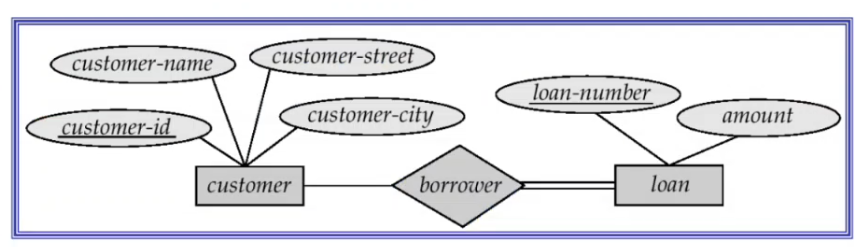
\includegraphics[width=0.7\linewidth]{img/scsreenshot001}
		\caption{参与约束}
		\label{fig:scsreenshot001}
	\end{figure}
	\item 三角形:自上而下的层级划分
\end{itemize}

\section{函数依赖FD}
\textbf{函数依赖的定义}:$\alpha\rightarrow\beta$即$ \alpha $的值决定了$ \beta 
$的值。

\textbf{Trivial无意义和Non-Trivial}:
\begin{itemize}
	\item 无意义函数依赖Trivial:AB$\rightarrow$A
	\item 有意义Non-Trivial:AB$\rightarrow$C
\end{itemize}

\textbf{FD和key的关系}
\begin{itemize}
	\item $ \alpha $是R的超键$\Leftrightarrow \alpha \rightarrow$R
	\item $ \alpha $是R的候选键$\Leftrightarrow \alpha \rightarrow$R且没有$ 
	\beta $ \textit{s.t.} $ \beta \subset \{\alpha, \beta\} \rightarrow$R
\end{itemize}

\textbf{闭包与最小依赖集}:见下图\hyperref[fig:dsjalscreenshot001]{手写笔记}。
\begin{figure}[th]
	\centering
	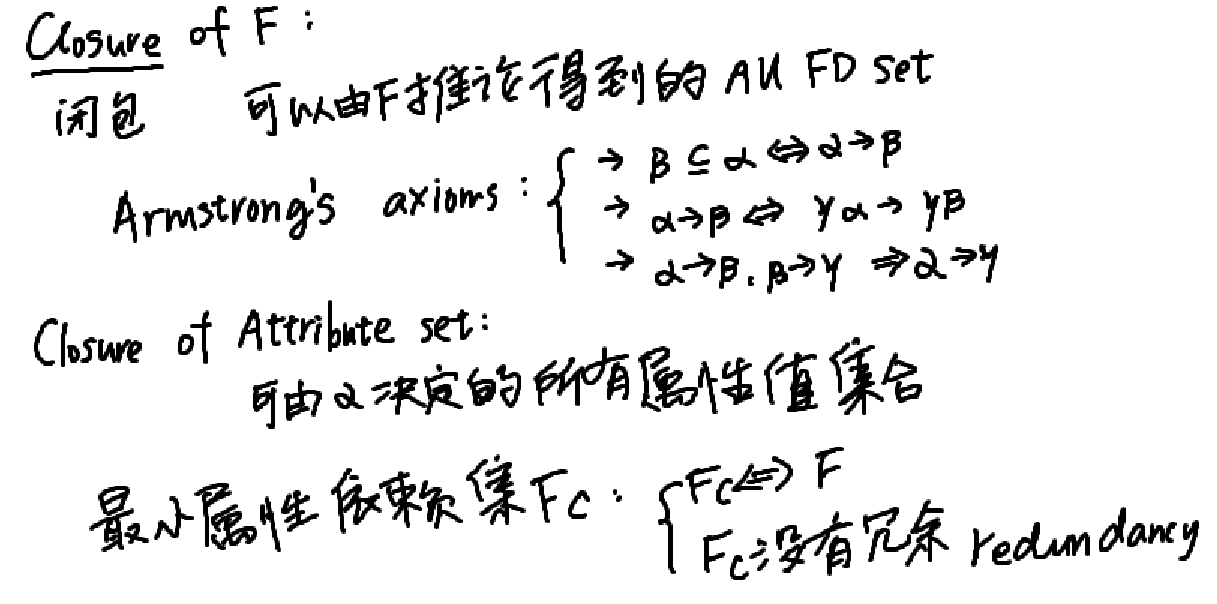
\includegraphics[width=1\linewidth]{img/dsjalscreenshot001}
	\caption{闭包与最小依赖集手写笔记}
	\label{fig:dsjalscreenshot001}
\end{figure}

\section{关系型数据库设计:3NF}
数据库异常行为包括函数依赖下的冗余存储、异常更新、异常插入、异常删除,如下图(position$\rightarrow$salary)。
\begin{figure}[ht]
  \centering
  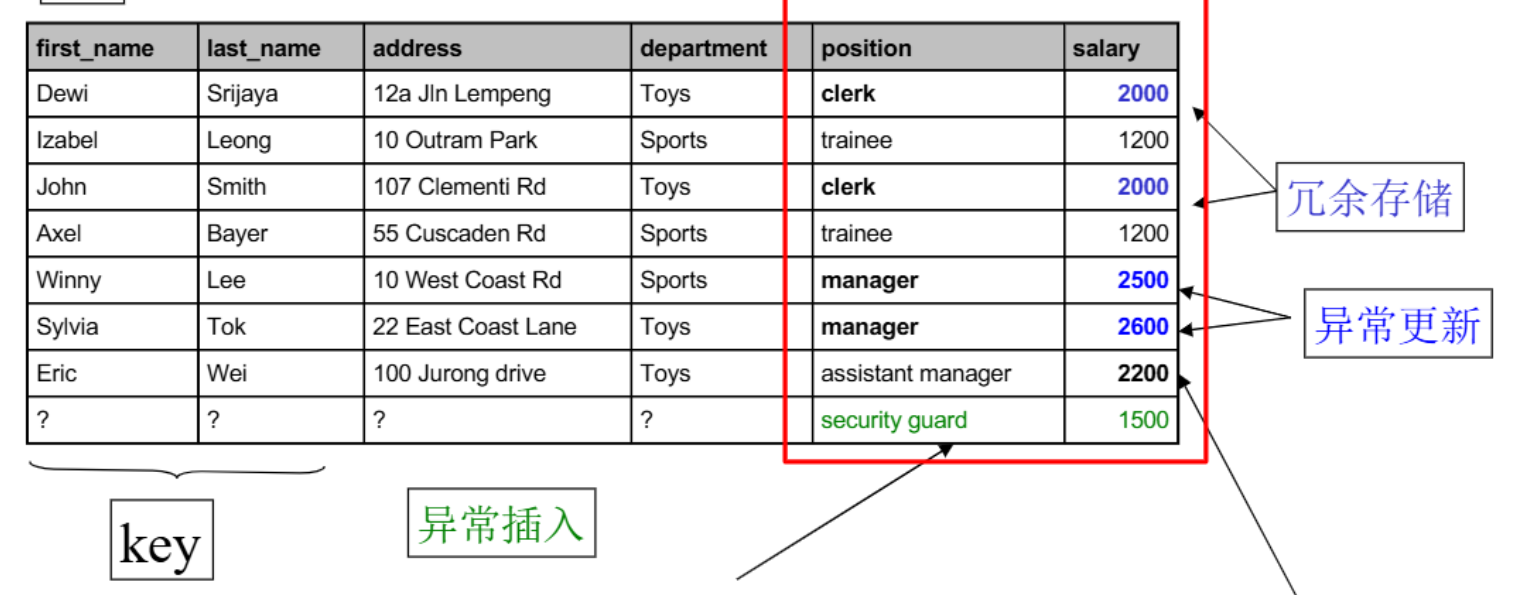
\includegraphics[width=0.8\linewidth]{img/屏幕截图 2024-11-04 112858.png}
  \caption{数据库异常行为}
  \label{fig:my_label}
\end{figure}

\textbf{规范化}是将关系型数据库分解的过程。$\mathbf{R}=R_1, R_2, \dots, R_n$。
\begin{itemize}
    \item 要求分解无损、依赖保留且冗余信息小。
\end{itemize}

\textbf{依赖保留}:FDs存在于各个单个relation,以便于验证FD。
\begin{itemize}
    \item 即,所有子表格FD并集的闭包与原来表格FD闭包一致
\begin{smallmdframed}
    给定一组函数依赖 $F$,$F$ 的闭包记作 $F^+$,它是所有由 $F$ 逻辑上蕴涵的函数依赖的集合。换句话说,$F^+$ 包括 $F$ 中的所有函数依赖以及可以通过 $F$ 中的函数依赖使用推理规则推导出来的所有函数依赖。

    计算一个属性集 $X$ 关于一组函数依赖 $F$ 的闭包 $X^+$ 的方法如下:

    \begin{enumerate}
    \item {初始化}:设 $X^+$ 为 $X$ 的初始值。
    \item {迭代}:重复以下步骤直到 $X^+$ 不再变化:
        \begin{itemize}
            \item 对于每一个 $F$ 中的函数依赖 $A \rightarrow B$,
                \begin{itemize}
                    \item 如果 $A \subseteq X^+$,则将 $B$ 添加到 $X^+$ 中。
                \end{itemize}
        \end{itemize}
    \end{enumerate}

    当 $X^+$ 不再变化时,算法结束,此时 $X^+$ 就是 $X$ 在 $F$ 下的闭包。
\end{smallmdframed}
\end{itemize}

\textbf{不满足依赖保留的分解:}
\begin{itemize}
    \item 可能会出现信息丢失、存储冗余等问题。
    \item 如果不能通过自然连接而恢复依赖,则出现信息丢失。
    \item 在下图中,$R_1$和$R_2$不存在依赖$B\rightarrow C$。
\begin{figure}[ht]
    \centering
    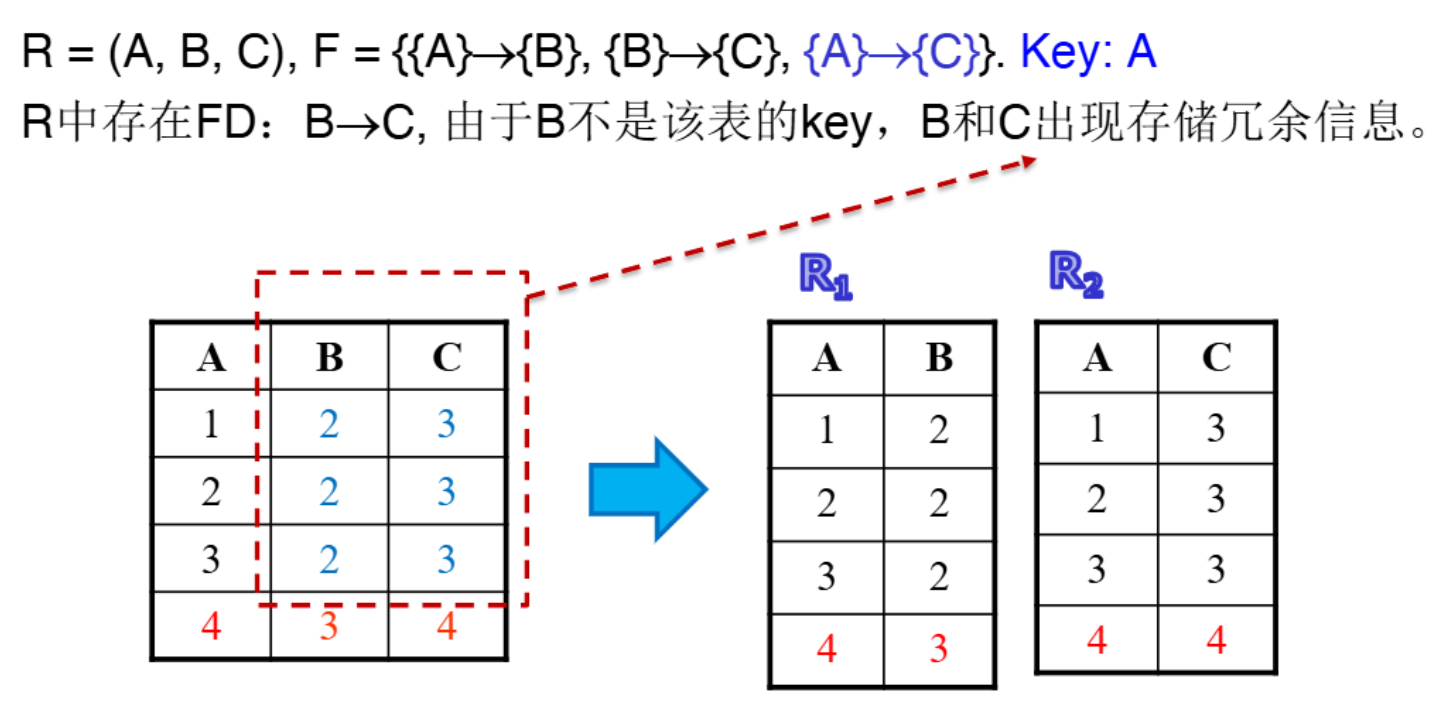
\includegraphics[width=0.7\linewidth]{img/屏幕截图 2024-11-04 134914.png}
    \label{fig:my_label}
    \caption{错误分解}
\end{figure}
    \item $F_1=\{\{A\}\rightarrow\{B\}\}\&F_2=\{\{A\}\rightarrow\{C\}\}, ({F_1}\cup{F_2})^+\neq{F}^+$。正确分解如图3。
\begin{figure}[ht]
  \centering
  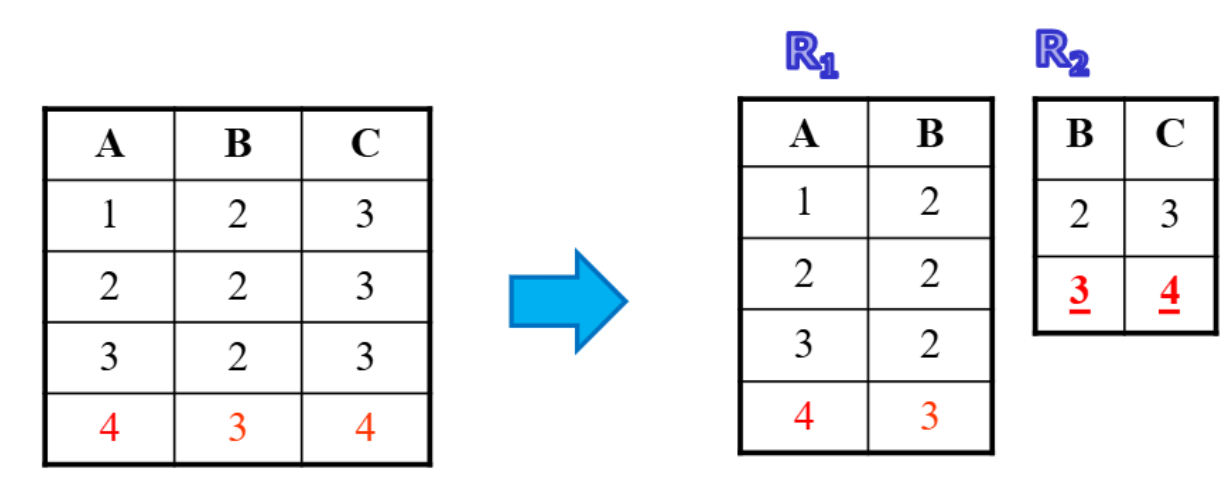
\includegraphics[width=0.6\linewidth]{img/屏幕截图 2024-11-04 141626.png}
  \caption{正确分解}
  \label{fig:my_label}
\end{figure}
\end{itemize}

\textbf{Lossless Join Decomposition:} 
\begin{itemize}
    \item 如果能利用分解后的表恢复原来的表,则该分解是无损的。
    \item 两个schema的交集属性至少构成其中一个schema的key。
    \begin{itemize}
        \item 外键必须引用另一个表的候选键。
    \end{itemize}
\end{itemize}

\textbf{1NF:第一范式}
\begin{itemize}
    \item 第一范式:表中所有属性的域没有多值属性。
    \item 根据关系模型的定义,关系表(relational tables)永远是1NF。
    \begin{itemize}
        \item 关系模型要求每一个属性都是原子的。
    \end{itemize}
\begin{smallmdframed}
1NF是不够的,不一定能满足无损、依赖保留和形式良好。
\\ 范式是对关系模式的规范化,不是对分解方法的选择。
\end{smallmdframed}
\end{itemize}

\textbf{2NF:第二范式}
\begin{itemize}
    \item 定义:1NF基础上,所有非主属性完全函数依赖于任何一个候选键。
    \begin{itemize}
        \item 2NF确保所有非主属性完全依赖于任何一个候选键,而不是部分依赖于候选键的一部分。即,非主属性必须完全依赖于候选码。
        \item 2NF通过消除部分函数依赖,可以减少数据冗余,提高数据的一致性和完整性。
    \end{itemize}
    \item 形式化:$R$ 是在 2NF 中当且仅当对于每个函数依赖 $X \rightarrow \{A\}$ 在 $F^+$ 中,至少满足以下三个条件的其中一条:
    \begin{itemize}
        \item $A \in X$(函数依赖是平凡的):自己依赖自己,无函数依赖
        \item $X$ 不是某个候选键的真子集:被依赖属性非为部分候选键
        \item $A$ 是一个主属性
    \end{itemize}
    \item 向2NF的转换:
    \begin{itemize}
        \item 如果存在非主属性对候选码的部份依赖,则这个属性和主关键字这一部分应该分离开作为一个新表。
    \end{itemize}
\begin{smallmdframed}
假设关系模式 $R(A, B, C, D)$,$(A, B)$ 是主键,函数依赖集为 $F = \{A \rightarrow C, (A, B) \rightarrow D\}$。

\begin{itemize}
        \item 主键是 $(A, B)$。
        \item 非主属性是 $C$ 和 $D$。
        \item 函数依赖 $A \rightarrow C$ 表明 $C$ 部分依赖于主键 $(A, B)$ 的一部分 $A$。
        \item 函数依赖 $(A, B) \rightarrow D$ 表明 $D$ 完全依赖于主键 $(A, B)$。
\end{itemize}
结论:关系模式 $R$ 不满足2NF,因为存在部分函数依赖 $A \rightarrow C$。
\\转换为2NF:
\begin{itemize}
    \item 分离成为两个关系模式$R_1(A,C)$和$R_2(A,B,D)$。
    \item $R_1$和$R_2$的FDs,非主属性都完全依赖于主键。
\end{itemize}
\end{smallmdframed}
\end{itemize}


\textbf{3NF:第三范式}
\begin{itemize}
    \item 定义:在1NF的基础上,任何非主属性不依赖于非键。
    \begin{itemize}
        \item 理解:在2NF的基础上消除传递依赖。
        \item 3NF同样减少数据冗余和提高数据的一致性。
    \end{itemize}
    \item 形式化:$R$ 是在 3NF 中当且仅当对于每个函数依赖 $X \rightarrow \{A\}$ 在 $F^+$ 中,至少满足以下三个条件的其中一条:
    \begin{itemize}
        \item $A \in X$(函数依赖是平凡的)。
        \item $X$ 是R的超键。(相比起2NF的更进一步。)
        \item $A$ 是一个主属性。
    \end{itemize}
    \item 3NF的分解:假设有一个关系模式 \( R(A, B, C, D) \),其函数依赖集为 \( F = \{A \rightarrow B, B \rightarrow C, A \rightarrow D\} \)。
    \begin{itemize}
        \item {确定候选键}:计算属性闭包,发现 \( A \) 是候选键,因为 \( A^+ = \{A, B, C, D\} \)。
        \item {识别非主属性}:非主属性是 \( B \)、\( C \) 和 \( D \)。
        \item {检查传递依赖}:存在传递依赖 \( A \rightarrow B \rightarrow C \),因为 \( A \rightarrow B \) 且 \( B \rightarrow C \),但 \( A \not\rightarrow C \)。
        \item {分解关系模式}:将 \( R \) 分解为两个关系模式:\( R_1(A, B, D) \)和\( R_2(B, C) \)
    \end{itemize}
\begin{smallmdframed}
    一个值得注意的自环传递例子:
    \begin{itemize}
        \item $R=(B,C,E)$,$F = \left\{ \{{E}\} \to \{{B}\}, \; \{{B,C}\} \to \{{E}\} \right\}$
        \item 找出候选键:BC和EC。
        \item 满足任何非主属性不依赖于非键。
        \item 该关系模式符合3NF范式。
    \end{itemize}
\end{smallmdframed}
\end{itemize}

\textbf{BCNF:Boyce-Codd范式}
\begin{itemize}
    \item BCNF旨在消除非平凡的多值依赖和非主属性对候选键的部分依赖。
    \item 形式化:$R$ 是在 BCNF 中当且仅当对于每个函数依赖 $X \rightarrow \{A\}$ 
    在 $F^+$ 中,至少满足以下两个条件的其中一条:
    \begin{itemize}
        \item $A \in X$(函数依赖是平凡的)。
        \item $X$ 是R的超键。
    \end{itemize}
    \item 就是说$\rightarrow$对于任意一个non-trivial函数依赖,左侧为超键。\\
    非候选键不能决定其它属性。
\end{itemize}

\section{内存层级和文件组织$_{377}$}

\textbf{磁盘和主存}
\begin{itemize}
	\item DBMS将信息存储在磁盘上。
	\item 数据才磁盘上的存储单元为块(block),又称为页(page)。
	\item 当前使用的数据存储在主存,主要数据存储在二次存储,旧数据存储在磁带。
\end{itemize}

\textbf{文件组织}
\begin{itemize}
	\item 文件组织引入:
	\begin{itemize}
		\item 在数据库存储中,一个文件相当于一个表,即relation实例。
		\item 表格中的一行,文件中的一个元组即一个记录。
		\item 一个表格中的记录大小是固定的。
	\end{itemize}
	\item 如何组织记录存放在文件里?
	\begin{figure}[th]
		\centering
		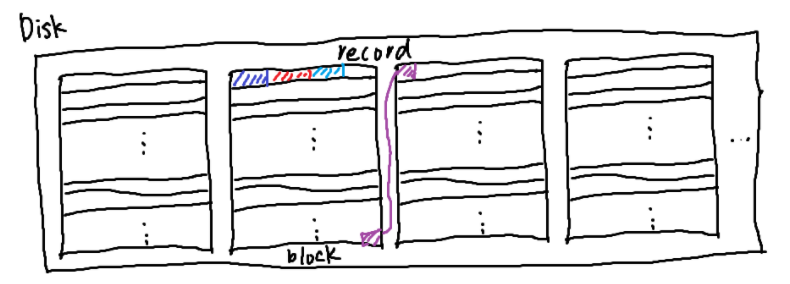
\includegraphics[width=0.7\linewidth]{img/db2}
		\caption{文件组织}
		\label{fig:db2}
	\end{figure}
	
	\begin{itemize}
		\item 固定长度记录:
		存储记录为连续的固定区域存储。同个文件的记录可能跨block存储。删除记录需要内存空
		间移位并且利用free list回收空间。
		\begin{smallmdframed}
			{Free list}:空闲记录链表,在文件首部指向第一个删除记录的位置。
		\end{smallmdframed}
		\item 可变大小记录:存储变长几里路,并且允许记录中某个字段重复出现。
	\end{itemize}
\end{itemize}

\textbf{如何存储可变大小记录?}
\begin{itemize}
	\item 方法一:用字节字符标识记录结尾。
	\begin{itemize}
		\item 删除困难且插入困难。
	\end{itemize}
	\item 方法二:预先分配最大的可能长度,插入记录时用符号$ \bot $填充末尾部分
	\item 方法三:指针方法:设置两种结构来组织文件:锚定块和溢出块。
	\begin{itemize}
		\item 对于具有重复属性的记录类型很有效。
		\item 锚定块\textit{Anchor}:包含链的第一条记录
		\item 溢出块\textit{Overflow}:溢出字段
	\end{itemize}
\end{itemize}

\textbf{文件中记录的组织方式}
\begin{itemize}
	\item Heap堆:无序存放,有空间就可以存放
	\begin{itemize}
		\item 需要记录的信息:每个文件存放在哪些页面、页面的剩余空间、每个页面存放了记
		录
		的位置信息。\hfill\textit{处理好文件和页面之间的关系}
	\end{itemize}
	\item Sequential有序:按某个搜索键的值的顺序存放
	\begin{itemize}
		\item 删除:用指针跳过该记录
		\item 插入:找到插入位置$\rightarrow$如果有可用空间就插入||如果没有可用空间就
		插入到溢出块中。
		\item 时不时重新组织文件以恢复顺序
	\end{itemize}
	\item Hashing哈希:计算哈希值并指向块
	\begin{itemize}
		\item 设计适合文件大小的哈希函数。比如假设我们为$ R $分配1200个页面,我们可用
		设计以某个合适属性值的模1200作为哈希寻址函数。
		\item 如果该页面已满,就创建一个溢出页面并在那里创建记录。
		\item 不适用于范围搜索。
	\end{itemize}
\end{itemize}

\textbf{时间成本分析}:
\begin{itemize}
	\item 以磁盘读写page的总次数作为衡量单位。
	\item 假设$ B $为文件的数据pages数量:
	\begin{figure}[th]
		\centering
		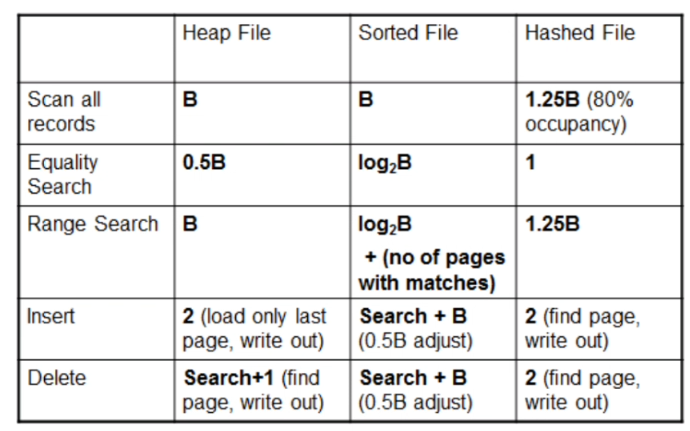
\includegraphics[width=0.7\linewidth]{img/screedsahkjnshot001}
		\caption{文件存储方式时间成本分析}
		\label{fig:screedsahkjnshot001}
	\end{figure}
	\item Hash扫描所有文件的成本较高。
	\item Hash查询特定文件的成本最低,其次是有序存储。
	\item 范围查找Hash成本最高,有序查找最低,
	\item 插入操作有序的成本非常高。
	\item 插入和删除Hash都很方便,删除的话直接删除比有序删除方便很多(不重排)。
\end{itemize}

\textbf{数据字典}:即系统目录,存放元数据。
\begin{itemize}
	\item {关系表的信息}:
	\begin{itemize}
		\item names of relations关系名称
		\item names and types of attributes of each relation属性值名称和类型
		\item names and definitions of views视图名称和定义
		\item integrity constraints约束
	\end{itemize}
	\item {用户账号信息},包括密码。
	\item {统计和描述性数据}:
	\begin{itemize}
		\item number of tuples in each relation关系元组数量
	\end{itemize}
	\item {物理的文件组织信息}:
	\begin{itemize}
		\item How relation is stored (sequential/hash/...)关系存储方式
		\item Physical location of relation:物理存储地址
		\begin{itemize}
			\item operating system file name or $\downarrow$
			\item disk addresses of blocks containing records of the relation
		\end{itemize}
	\end{itemize}
	\item {索引信息(index)}
\end{itemize}


\section{索引的相关概念$_{405}$}

\textbf{索引的引入}
\begin{itemize}
    \item ID排序+二分搜索:$\log(n)$。
    \item ID排序+索引条目:$<ID, page.No>$\lstinline{[Search-key|pointer]}
    \begin{itemize}
        \item 每个page的第一条记录有一个条目,从而反映条目区间。
        \item 对索引使用二分查找。
        \item 可以创建多级索引Multilevel Index。
    \end{itemize}
    \item 两种基础索引类型:顺序索引、哈希无序索引。
\end{itemize}

\textbf{顺序索引}
\begin{itemize}
    \item 顺序索引也成为树索引。
    \item 获取一个记录所需的page访问次数为\lstinline{tree.height+1}
\begin{figure}[ht]
  \centering
  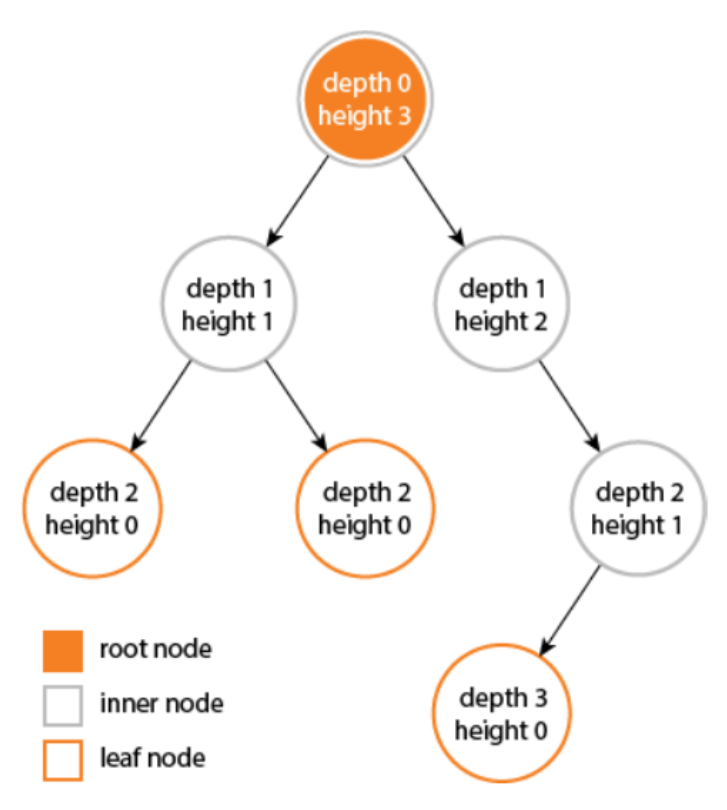
\includegraphics[width=0.3\linewidth]{img/屏幕截图 2024-11-05 142036.png}
  \caption{tree index}
  \label{fig:my_label}
\end{figure}
\end{itemize}
    
\textbf{主索引和辅助索引}
\begin{itemize}
    \item 主索引{Primary index}:文件实际存放也是按照search key 排序的。其基于主键或唯一标识符构建索引,具有唯一性。
    \item 辅助索引{Secondary index}:也称为二级索引。文件的实际存放不按照search key 排序。其基于非主属性构建索引,不具有唯一性。
    \\ 1. 当检索许多记录时,辅助索引昂贵,因为磁盘不连续寻址耗时长。
    \\ 2. 辅助索引常用于优化不涉及主键的查询。
    \begin{smallmdframed}
        对于非排序属性(如账号、余额等),可以通过额外建立索引生成二级索引,从而提高查询效率。这样可以在不需要重新组织数据的情况下,实现对这些属性的有效查询。
    \end{smallmdframed}
\end{itemize}

\textbf{稀疏索引和密集索引} 
\begin{itemize}
    \item 稀疏索引Sparse Index:仅包含某些search key。
    \\稀疏检索:找到最后一个比K小key的index,然后向后遍历寻找K。
    \item 密集索引Dense Index:包含所有search key。
    \begin{figure}[ht]
        \centering
        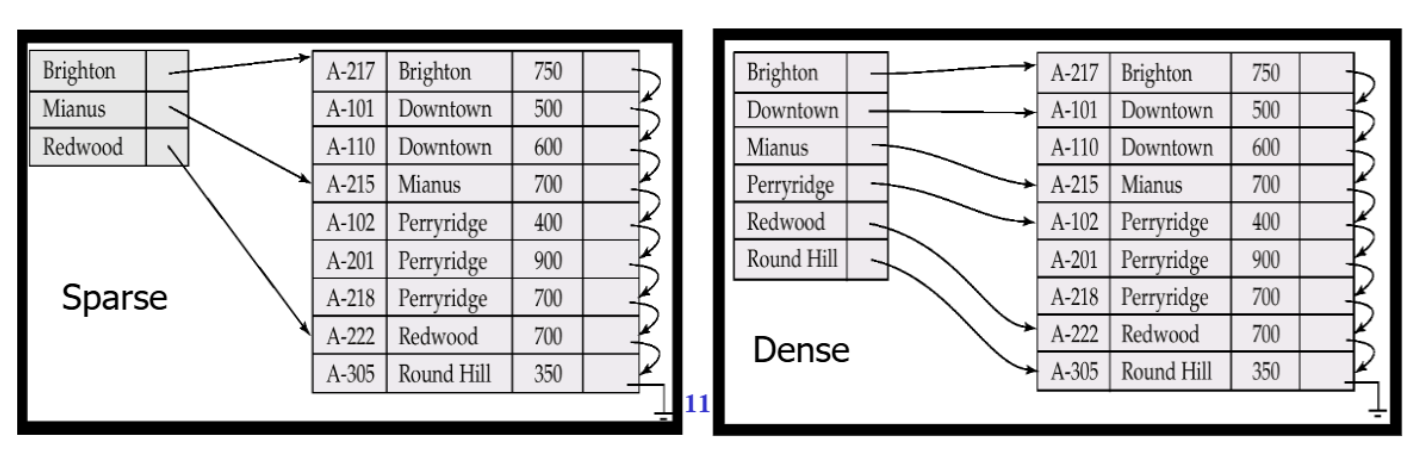
\includegraphics[width=0.7\linewidth]{img/image.png}
        \caption{稀疏索引和密集索引}
        \label{fig:my_label}
    \end{figure}
\end{itemize}

\textbf{哈希索引}
\begin{figure}[ht]
  \centering
  \begin{minipage}[b]{0.5\textwidth}
    \centering
    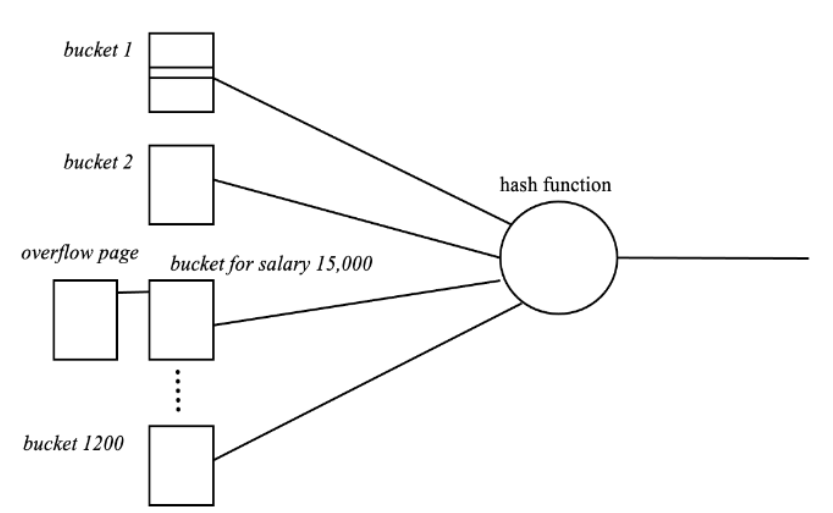
\includegraphics[width=\linewidth]{img/屏幕截图 2024-11-05 160116.png}
    \caption{哈希索引结构}
    \label{fig:hash_structure}
  \end{minipage}%
  \hfill
  \begin{minipage}[b]{0.5\textwidth}
    \centering
    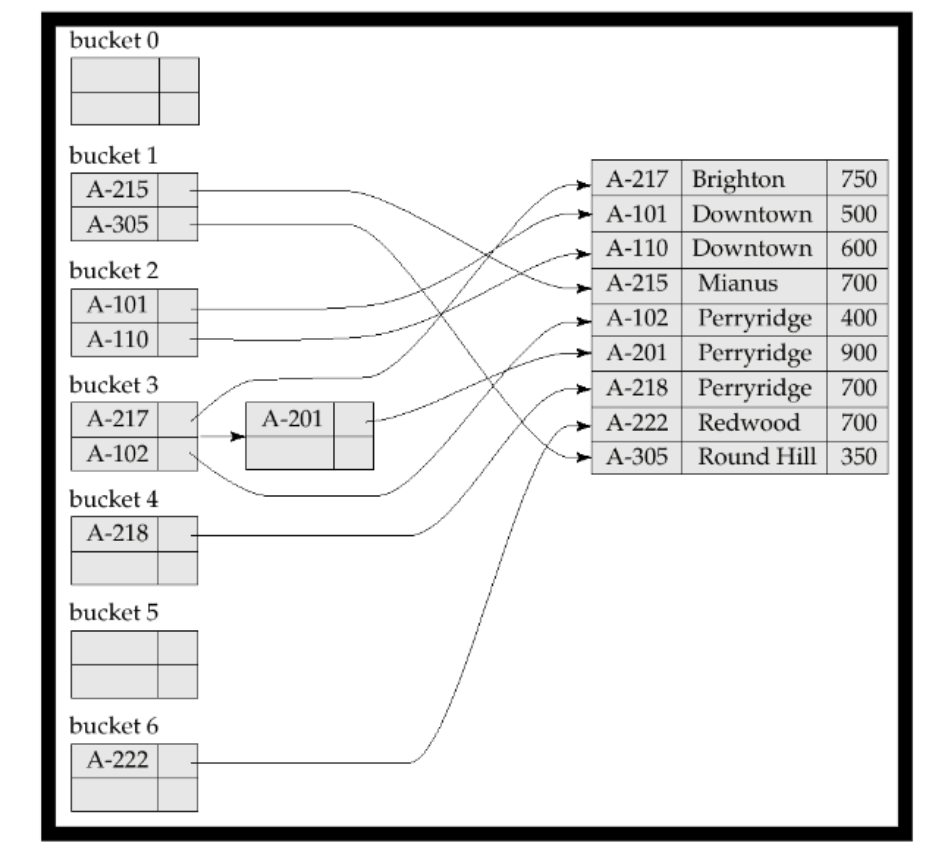
\includegraphics[width=0.8\linewidth]{img/屏幕截图 2024-11-05 161453.png}
    \caption{哈希索引示例}
    \label{fig:hash_example}
  \end{minipage}
\end{figure}
\begin{itemize}
    \item 哈希索引维护哈希函数\lstinline{F(search key)=location_of_record}
    \item 严格来说,哈希索引是二级索引(辅助索引)。
\end{itemize}

\textbf{索引的评价指标}
\begin{itemize}
    \item 成本定义为最坏情况下的磁盘打开页数。
    \item 高效支持不同查询:例如,辅助索引(包括哈希)在范围检索表现很差,因为磁盘经常需要跨区寻址。
    \item 更新时间成本小:当文件被修改时,索引也必须更新。
    \item 额外存储成本小(即index本身的大小):索引的大小应该比数据文件小得多。
\end{itemize}

\textbf{索引的更新}
\begin{itemize}
    \item 删除:索引的删除思路符合直觉。
    \begin{itemize}
        \item 如果删除的记录为索引的唯一记录,则对应的索引也要删除。
        \item 对于稀疏索引,如果删除记录的search key 在index存在,则将index里的的记录替换为所删除的下一条记录。如果下一条记录已经在index中存在,则直接删除。
    \end{itemize}
    \item 插入:同样符合直觉。
    \begin{itemize}
        \item 对于密集索引:如果search key没有出现在index则插入。
        \item 对于稀疏索引:
        \\1. 如果该索引为每个page维护有索引条目则不需要修改。
        \\2. 否则要创建新page。当有新的block(page)创建的时候,将block的第一个search key加入index。
    \end{itemize}
\end{itemize}

\section{索引进阶:$B^+$树和动态哈希}

\subsection{$B^+$树:}

\textbf{$B^+$树引入}
\begin{itemize}
    \item $B^+$树是一种特殊的平衡多路搜索树。
\begin{figure}[ht]
  \centering
  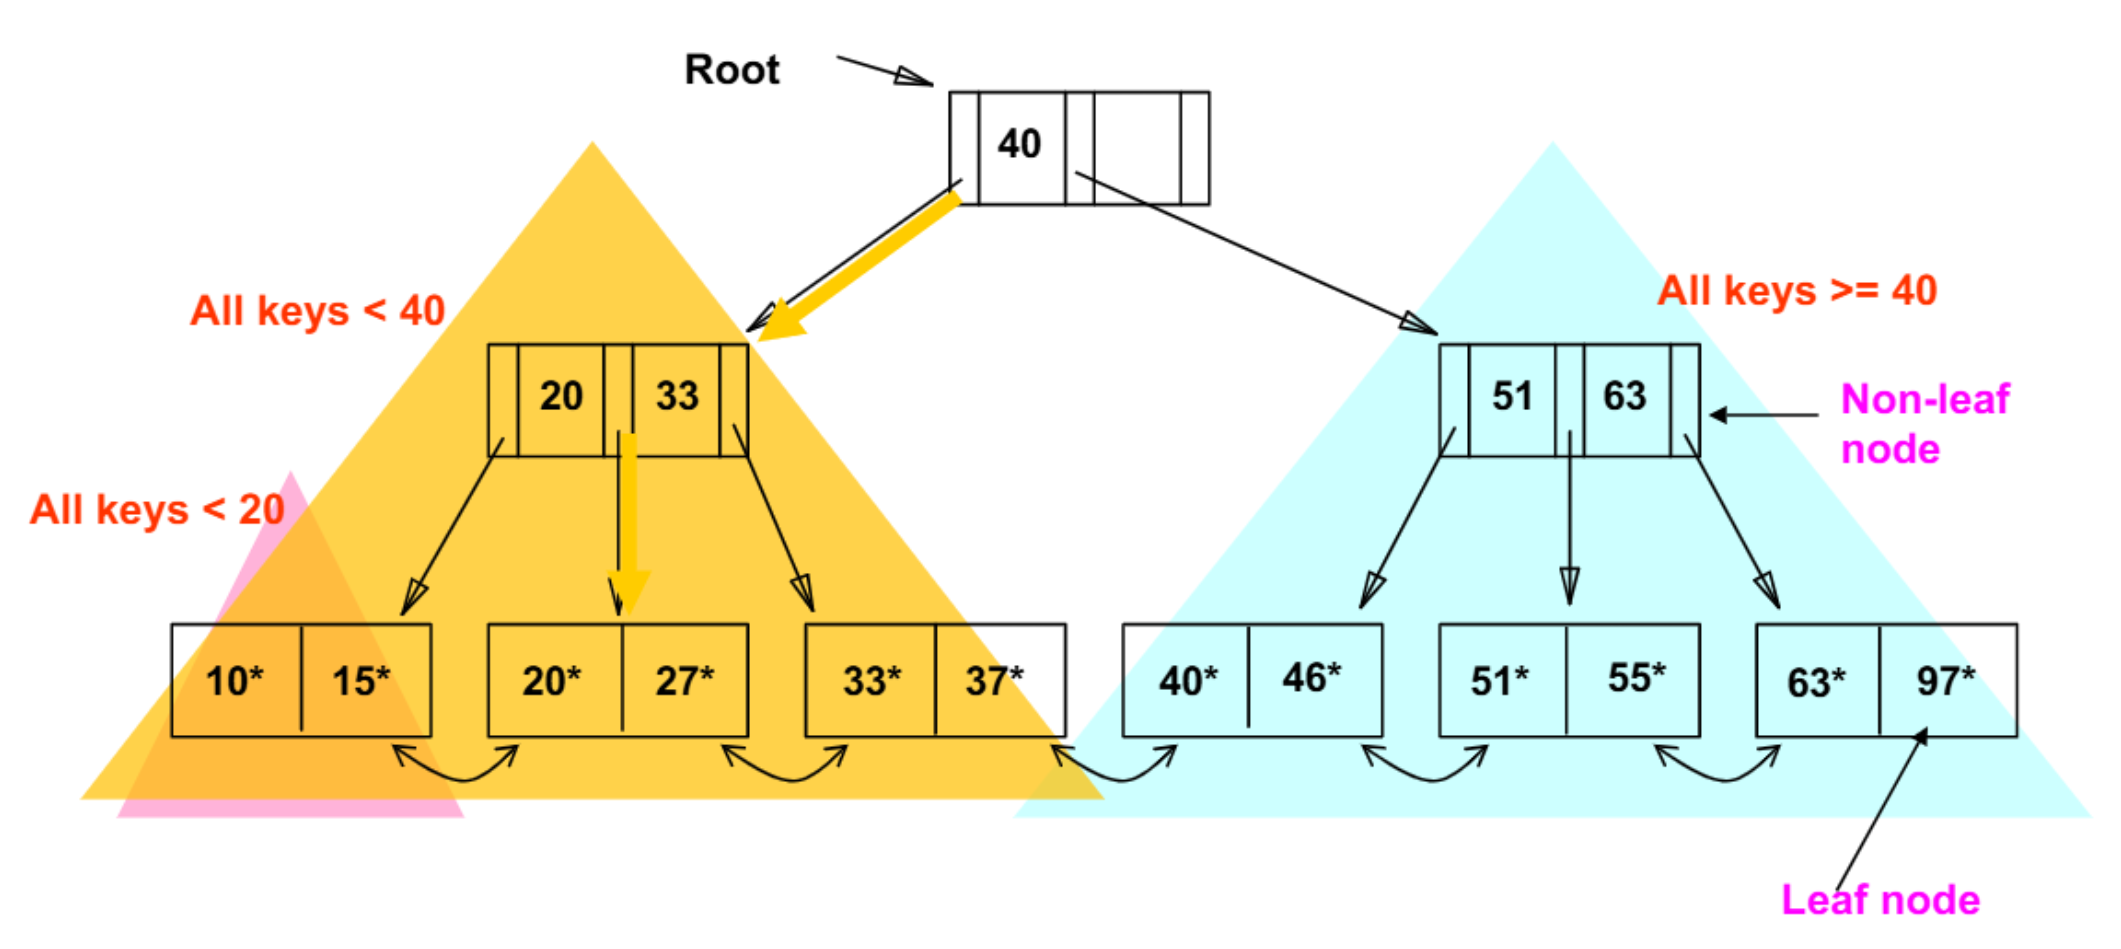
\includegraphics[width=0.7\linewidth]{img/屏幕截图 2024-11-05 190832.png}
  \caption{$B^+$树示意图}
  \label{fig:my_label}
\end{figure}
    \item $B^+$树是所有商业DBMS中优序索引的默认实现。
\end{itemize}

\textbf{$B^+$树的主要特征}
\begin{itemize}
    \item 所有叶子节点都在同一层。
    \item 非叶子节点只存储索引信息。
    \item 叶子节点存储实际数据信息。
    \item 叶子节点之间有指针连接:所有的叶子节点通过指针相互连接,形成一个双向链表。这种结构支持高效的范围查询和顺序扫描。
\end{itemize}

\textbf{$B^+$树的性质}
\begin{itemize}
    \item 从根到叶子的所有路径都具有相同的长度(a balanced tree)
    \item $n$ 称为扇出 fanout(每个节点最多可有拥有指针数):
    \begin{enumerate}
        \item 每个非叶节点都有数量在 $\lceil n/2 \rceil$ 到 $n$ 之间的指针
        \item 每个叶节点存储数量为 $\lceil (n-1)/2 \rceil$ 和 $n-1$ 之间的数据值
        \item 值 $\lceil (n-1)/2 \rceil$ 称为 order阶数(数据值的最小数量)
\begin{smallmdframed}
    1.和2. 都是在设定了子节点下限,从而维护树的平衡。
    \\特别例子:如果根不是叶节点,则至少有两个子节点。如果根是叶节点,可以有0到$(n-1)$个数据值。
\end{smallmdframed}
    \end{enumerate}
\end{itemize}
\begin{figure}[ht]
  \centering
  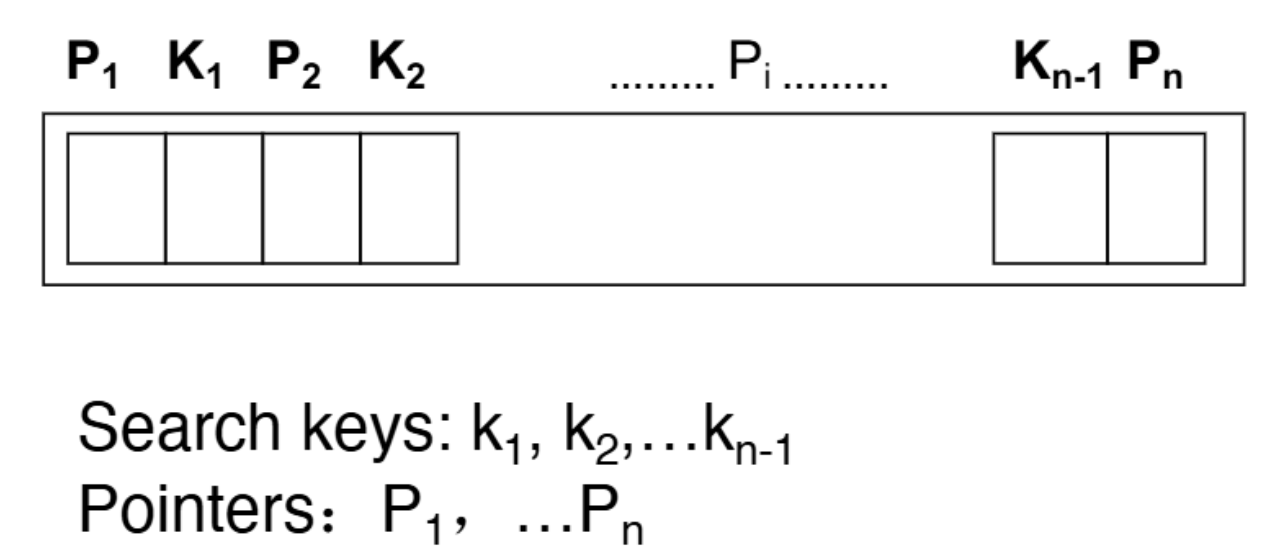
\includegraphics[width=0.6\linewidth]{img/屏幕截图 2024-11-05 194014.png}
  \caption{$B^+$树节点示意图}
  \label{fig:my_label}
\end{figure}

\textbf{$B^+$树查询}

\begin{itemize}
    \item 从所有记录中寻找$search\_{key}=a$的记录:
    \\从根节点开始:
    \begin{enumerate}
        \item 在当前节点内部寻找$P_i$,满足$K_{i-1} \leq a < k_i$。
        \item 跳到$P_i$指向的子节点。重复以上步骤直到叶节点。如果在叶结点中找不到,则该树不包含$search\_{key}=a$的记录。
    \end{enumerate}
\end{itemize}

\textbf{$B^+$树插入}
\begin{itemize}
    \item 用键值k进行查询,得到叶节点L。
    \item 将k插入到L中:
    \begin{enumerate}
        \item 如果L有空位,则插入完成。
        \item 如果L无空位:将L分裂成$L_1$和$L_2$:
        \begin{enumerate}
            \item 将keys平分(奇数则左侧多一个)。
            \item 更新L的父节点:插入$L_2$的最左侧数值。(中间键值往父节点插入)
            \item 如果父节点也无空位,则由下往上递归更新节点。
        \end{enumerate}
    \end{enumerate}
\begin{figure}[ht]
  \centering
  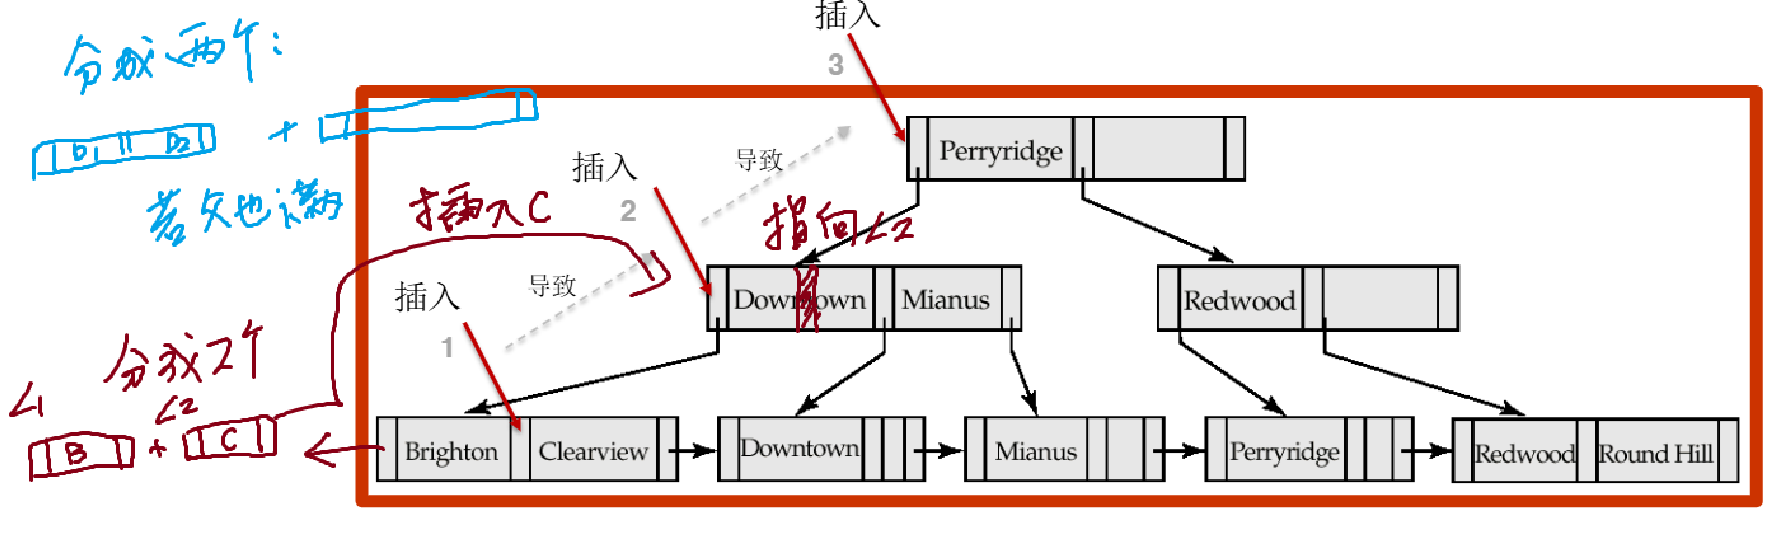
\includegraphics[width=\linewidth]{img/屏幕截图 2024-11-06 101536.png}
  \caption{$B^+$树插入}
  \label{fig:my_label}
\end{figure}
\end{itemize}

\textbf{$B^+$树删除}
\begin{itemize}
    \item 用k值查询,得到其所在叶节点L。
    \item 将k从L中移除:
    \begin{enumerate}
        \item 如果L有超过半数key,则结束。
        \item 否则,从右侧兄弟节点索取一个key。
        \begin{enumerate}
            \item 如果右侧节点少于$\lceil (n-1)/2 \rceil +1$个节点,则合并两个节点:
            \begin{itemize}
                \item 合并后,从L的父节点删除指向L的键值。
                \item 合并也可能发生连锁反映。
            \end{itemize}
        \end{enumerate}
    \end{enumerate}
\begin{figure}[ht]
  \centering
  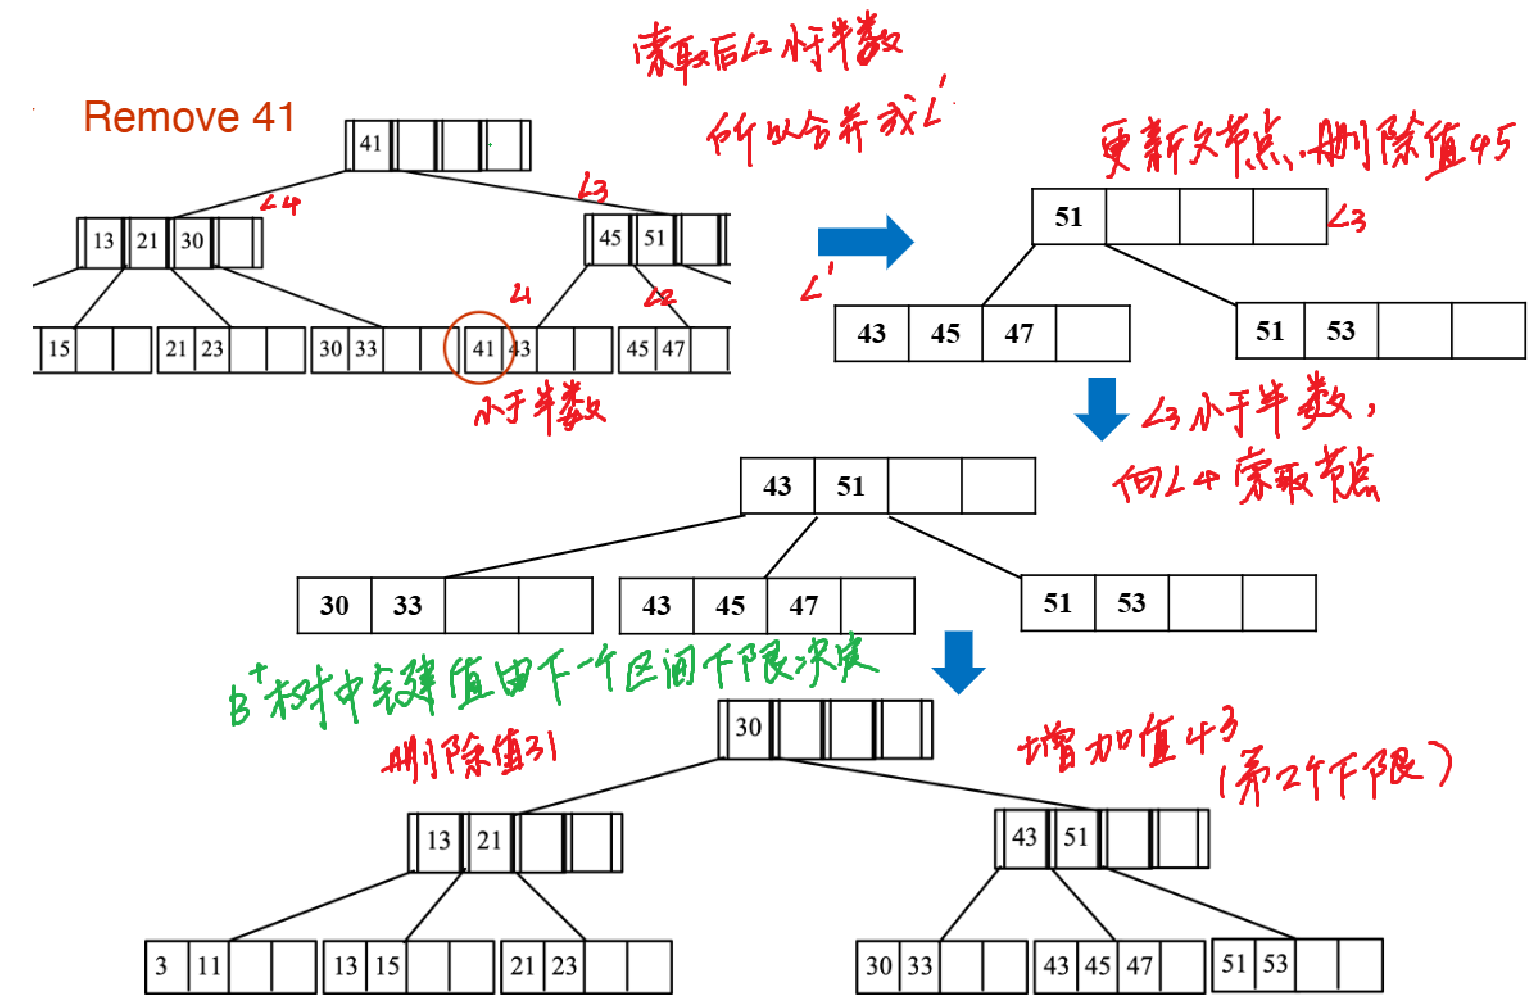
\includegraphics[width=0.8\linewidth]{img/屏幕截图 2024-11-06 103159.png}
  \caption{$B^+$树删除}
  \label{fig:my_label}
\end{figure}
\end{itemize}

\textbf{$B^+$树文件组织结构}
\begin{itemize}
    \item 可以用$B^+$树索引解决索引退化问题。
    \item 数据文件退化问题(碎片化)用$B^+$树来组织文件存储。要求:
    \begin{itemize}
        \item 叶节点存储数据本身。
        \item 叶节点存储的最大记录数小于非叶节点的最大指针数。
        \item (上面两条都是$B^+$树本身的要求)
    \end{itemize}
    \begin{smallmdframed}
        在文件组织和数据库管理中,索引退化(Index Degradation)是指索引结构在长时间运行和频繁的插入、删除操作后,逐渐失去其优化效果,导致性能下降的问题。索引退化会影响查询性能、增加磁盘I/O操作次数,并可能导致其他性能问题。
    \end{smallmdframed}
\begin{figure}[ht]
  \centering
  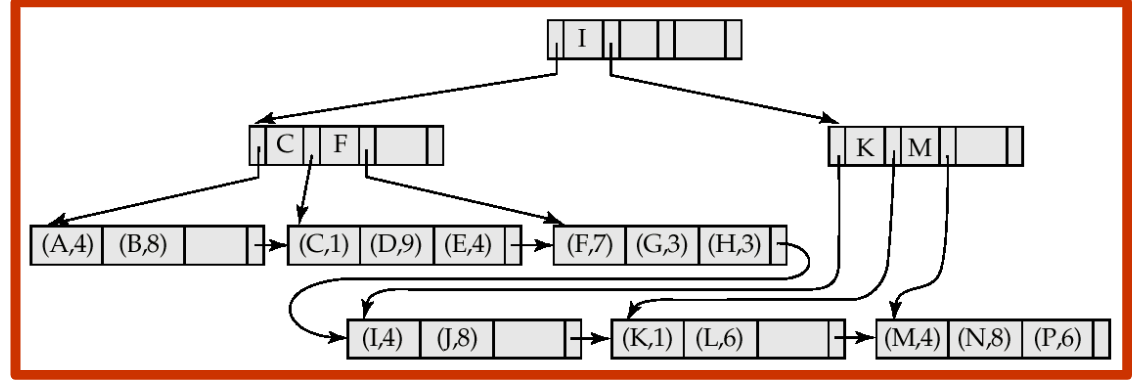
\includegraphics[width=0.7\linewidth]{img/屏幕截图 2024-11-06 104716.png}
  \caption{$B^+$树文件组织结构}
  \label{fig:my_label}
\end{figure}
\end{itemize}

\subsection{动态哈希:}

\textbf{静态哈希}:Buckets数量是固定的。将搜索键值固定映射到某个Bucket。随着数据增长,由于过多的溢出导致该index的性能退化。

\textbf{动态哈希}
\begin{itemize}
    \item Buckets数目可以动态调整。
    \item 关键:哈希结果和数据位置中间加一层指针:
    \begin{itemize}
        \item 使用指向buckets的指针目录,通过将目录加倍来增加buckets数量(见下)。
        \item 仅拆分溢出的存储bucket。
        \item 只需要对指针进行整理,成本小很多。
    \end{itemize}
\end{itemize}

\begin{figure}[ht]
  \centering
  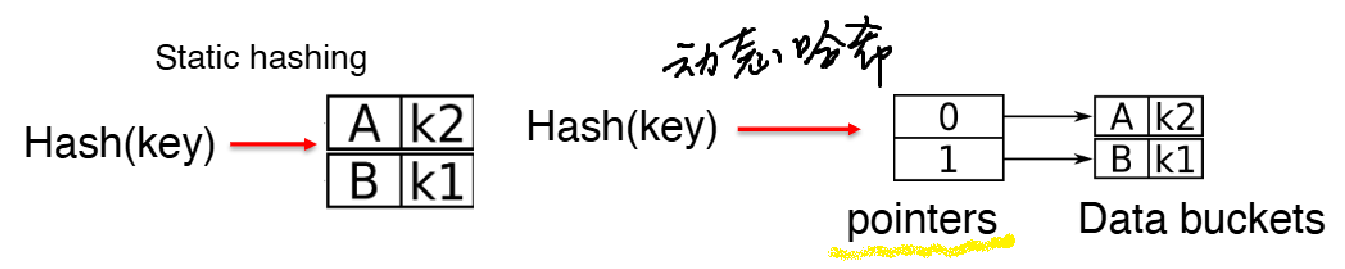
\includegraphics[width=0.8\linewidth]{img/屏幕截图 2024-11-06 112156.png}
  \caption{静态与动态哈希对比}
  \label{fig:my_label}
\end{figure}

\textbf{动态哈希函数的调整}
\begin{itemize}
    \item 掩码哈希:$f(value)=value\%(2^{DEPTH})$
    \item 通过全局深度$GLOBAL\ DEPTH$和局部深度$LOCAL\ DEPTH$动态分裂桶。
    \begin{itemize}
        \item 全局深度:将一个元素映射到一个桶时需要看几位。
        \item 局部深度:桶中所有元素相同尾数序列长度。
        \item $Global\ depth = \max\{Local\ depth\}$
        \item $Local\ depth = Global\ depth - \log_2{(lines)}$,其中$lines$为连接线段数量。
    \end{itemize}
\begin{figure}[ht]
  \centering
  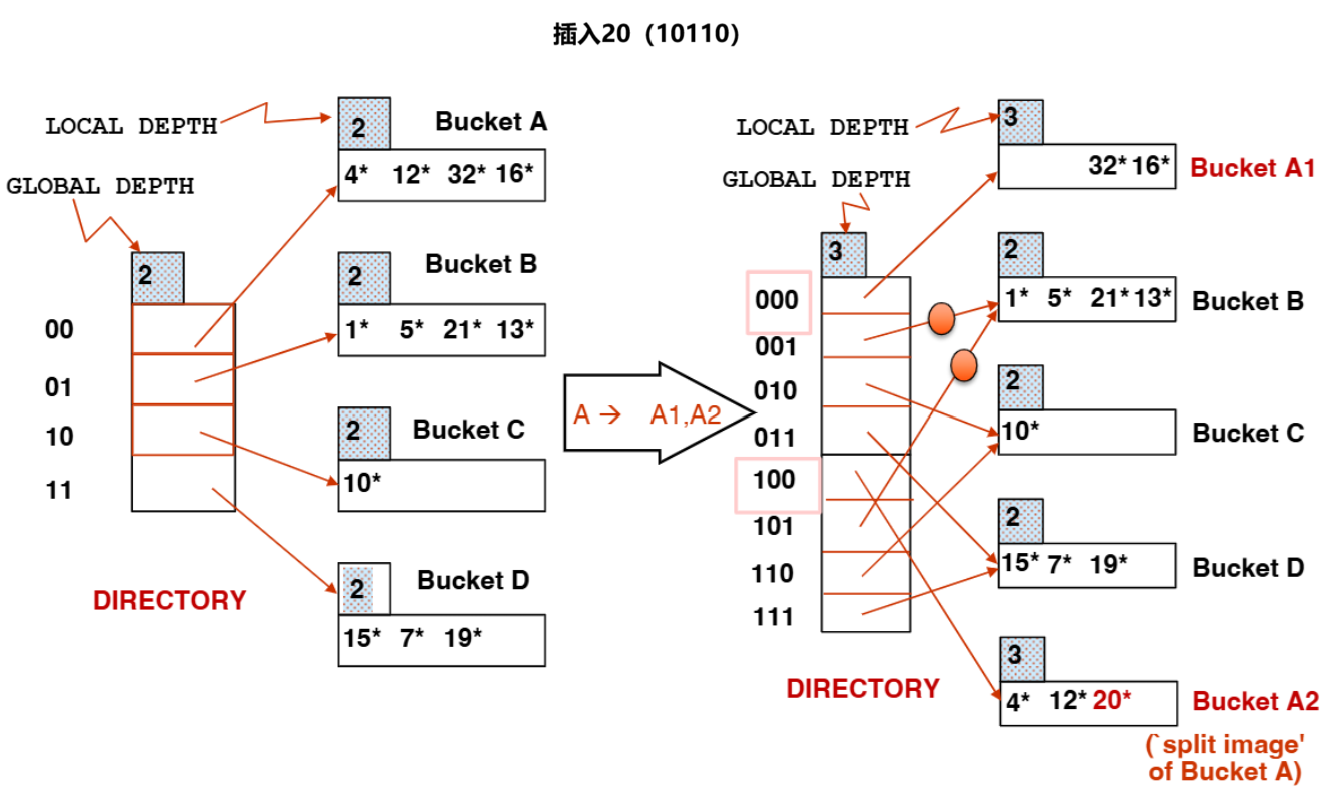
\includegraphics[width=0.7\linewidth]{img/屏幕截图 2024-11-06 134741.png}
  \caption{掩码哈希动态调整}
  \label{fig:my_label}
\end{figure}
\end{itemize}

\textbf{动态哈希删除}
\begin{itemize}
    \item 如果删除导致bucket变空,则将其与其镜像(譬如001和101)合并,合并后local depth-1。
    \item 当因为一系列删除操作,导致指针目录的任意指针与其镜像指针均指向同一个bucket,则将整体指针目录缩减一半,global depth-1。
\begin{figure}[ht]
  \centering
  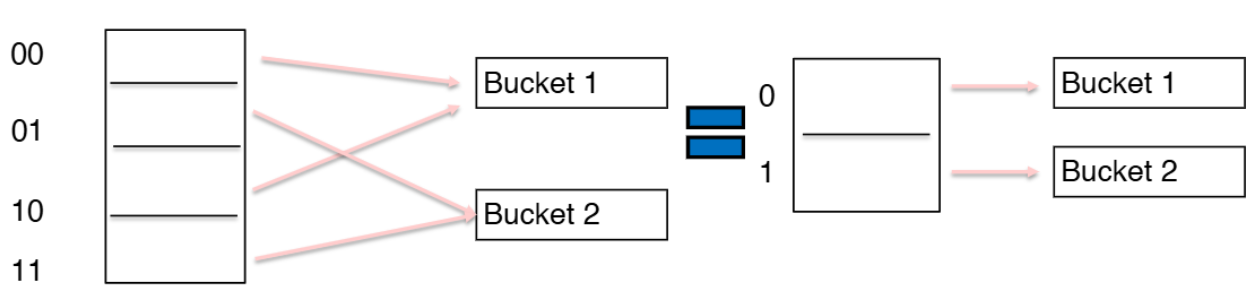
\includegraphics[width=0.8\linewidth]{img/屏幕截图 2024-11-06 135908.png}
  \caption{动态哈希全局目录缩减}
  \label{fig:my_label}
\end{figure}
\end{itemize}

\section{其它索引:多键访问}

\textbf{多键访问引入}
\begin{itemize}
	\item 如何加快具有多个条件的查询记录?
\begin{verbatim}
	Select loan-number
	From account
	Where branch-name<"Perryridge" and Balance = 1000
\end{verbatim}
	\item 策略一:先后查询\\
	先检查元组的branch-name然后在检查balance
	\item 策略二:交集查询\\
	先分别获取符合两种要求的指针,然后寻找指针的交集并获得记录。
\end{itemize}

\textbf{位图索引}
\begin{itemize}
	\item 位图索引(Bitmap)旨在对多个键同时进行高效查询。
	\item 引入:
	\begin{itemize}
		\item 记录按照顺序编号为$(R_0, R_1, R_2, \dots)$,给定$n$则检索$R_n$的效率
		很高。
		\item {仅对取值个数有限的属性特别适用。}
	\end{itemize}
	\item 最简单的形式:为属性(搜索键)的每个值都建有一个位图。
	\begin{itemize}
		\item 位图长度(bit个数)为record数量。
		\item 每个位图代表某个属性的某个值在记录中的取值情况。
	\end{itemize}
\begin{figure}[ht]
	\centering
	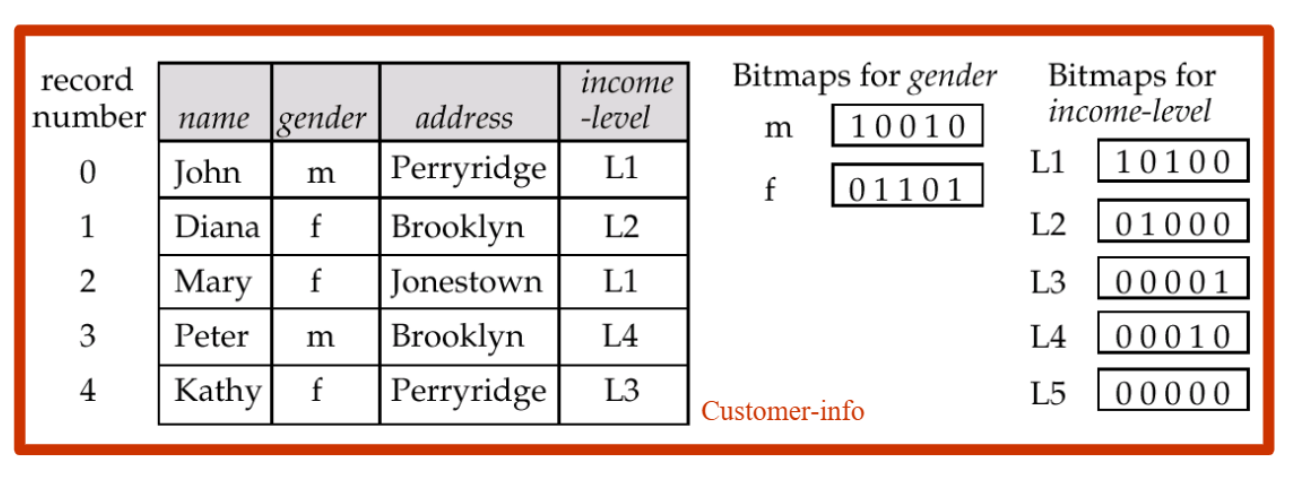
\includegraphics[width=0.7\linewidth]{img/屏幕截图 2024-11-06 190224.png}
	\caption{位图索引}
	\label{fig:my_label}
\end{figure}
\end{itemize}

\section{查询过程}

\textbf{查询过程的基本步骤}
\begin{enumerate}
	\item 解析和转化
	\begin{itemize}
		\item 将SQL查询语句转化为关系代数。
		\item 解析器检查语法和表名。
	\end{itemize}
	\item 求解
	\begin{itemize}
		\item 查询执行引擎采用查询评估计划,执行该计划并返回查询答案。
		\item 通过关于查询市场的统计数据制定更优的查询计划。
	\end{itemize}
\begin{figure}[ht]
	\centering
	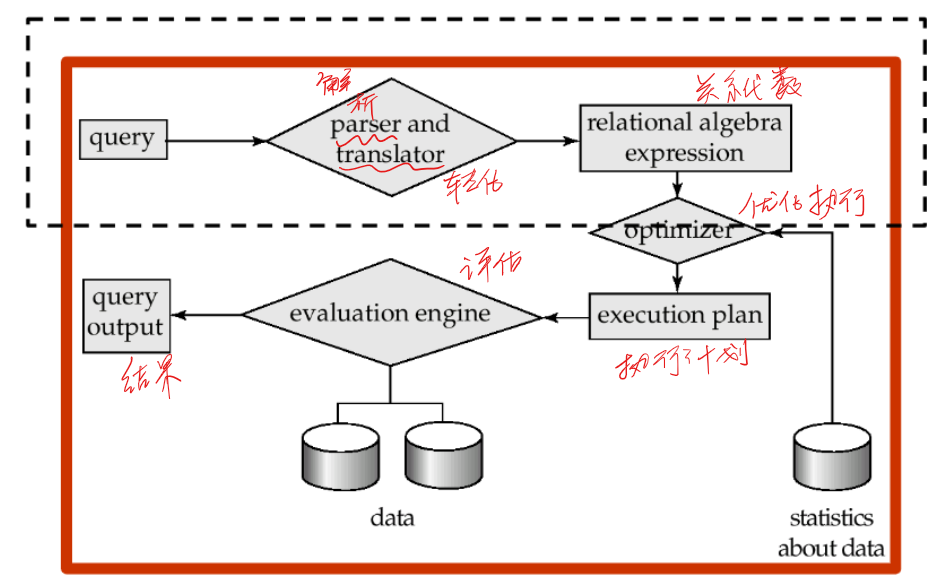
\includegraphics[width=0.7\linewidth]{img/屏幕截图 2024-11-06 191554.png}
	\caption{查询架构}
	\label{fig:my_label}
\end{figure}
\end{enumerate}

\textbf{优化引入和成本评估}
\begin{itemize}
	\item Need special evalution-plan to solve algebra expression.
	\begin{itemize}
		\item 关系代数表达式有许多等效表达式。
		\item 一个简单的关系运算可以有很多种算法实现。
		\item 例子:
		\begin{verbatim}
			select B,D
			from R,S
			where R.A='C' and S.E=2 and R.C=S.C
			#具有两种查询计划如下图所示。
		\end{verbatim}
	\begin{figure}[ht]
		\centering
		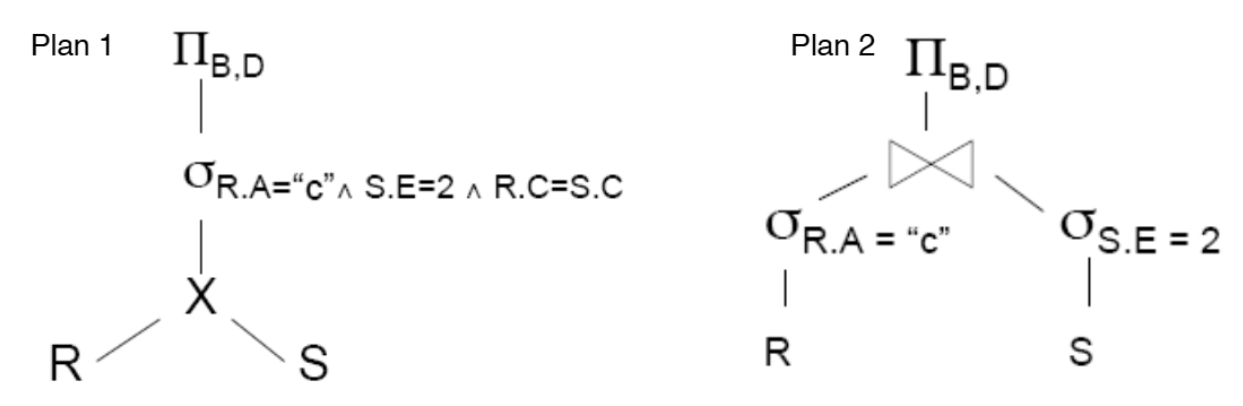
\includegraphics[width=0.7\linewidth]{img/屏幕截图 2024-11-06 193722.png}
		\caption{等价查询计划例子(查询语句见笔记)}
		\label{fig:my_label}
	\end{figure}
	\end{itemize}
	\item 把时间成本简单计算为:在磁盘和主存之间读写page的总数量。
	\begin{itemize}
		\item 忽略顺序I/O和随机I/O之间的成本差异(忽略寻道)。
		\item 忽略CPU成本。
		\item 忽略将最终结果写入磁盘的成本。
	\end{itemize}
	\item 时间成本页依赖于主存中缓冲区的大小,更多的内存可以减少磁盘访问的需求。
\end{itemize}

\textbf{选择操作的实现方式}:检索满足$\sigma_{A=V}(r)$的一些可能算法:
\begin{itemize}
	\item 算法一:线性搜索\hfill \emph{linear search}
	\begin{itemize}
		\item 访问每个page并测试所有记录是否满足条件。
		\item Cost estimate(扫描的磁盘页数)= $b_r$
		\begin{itemize}
			\item $b_r$标识包含关系表r中的记录的页数
			\item 如果选择条件是关于键key的,则一旦访问到目标记录查询便可停止。
			\item 平均成本为$\frac{b_r}{2}$
		\end{itemize}
	\end{itemize}
	\item 算法二:二分查找\hfill \emph{binary search}
	\begin{itemize}
		\item 在检索文件排序所依据的属性上适用。
		\item 假设该表的文件page是连续存储在磁盘上的。
		\item 成本估算:
		\begin{itemize}
			\item 定位一个元组的成本$\lceil \log_2(b_r) \rceil$
			\item 如果有多条记录满足选择条件,还需要算上跨越这些记录的page数。
		\end{itemize}
	\end{itemize}
	\item[$\Rightarrow$] 
	假设选择条件是\textbf{作用在搜索键上}的:算法三$\rightarrow$五
	\item 算法三:在候选键上的主索引\hfill \emph{primary tree index on candidate 
	key, equality}
	\begin{itemize}
		\item 检索满足相等条件的单个记录:Cost=$HT_i+1$ //$HT_i$为树的高度。
	\end{itemize}
	\item 算法四:在非键上的主索引\hfill \emph{primary tree index on non-key, 
	equality}
	\begin{itemize}
		\item 检索满足条件的多个记录,记录在连续的页面上。
		\item Cost = $HT_i+\text{包含检索记录的页数}$
	\end{itemize}
	\item 算法五:在搜索键上的二级索引\hfill \emph{equality on search-key of 
	secondary index}
	\begin{itemize}
		\item 如果搜索键是候选键,即检索单个记录:Cost=$HT_i+1$。
		\item 否则需要检索多个记录:Cost = $HT_i+\text{包含检索记录的页数}$。
		\begin{itemize}
			\item 记录可能位于不同的页面,成本昂贵。
			\item 最坏的情况:每条检索的记录都需要一页访问。
		\end{itemize}
	\end{itemize}
\begin{smallmdframed}
	如何区分搜索键和候选键:\hfill 主索引:文件按照search key存放
	\begin{itemize}
		\item 搜索键指的是查询的属性。\hfill 二级索引:不按照search key 存放,不唯一
		\item 候选键是关系表的属性,具有唯一性。
	\end{itemize}

\end{smallmdframed}
	\item[$\Rightarrow$] \textbf{涉及比较式}的查询:算法六$\rightarrow$七
	\item[$\rightarrow$] 实现$\sigma_{A\leq V}(r)$或$\sigma_{A\geq V}(r)$同样可以
	用线性扫描、二分搜索和索引。
	\item 算法六:主索引下的比较查询\hfill \emph{primary index, comparison}
	\begin{itemize}
		\item[$\rightarrow$] Relation is sorted on A.
		\item For $\sigma_{A\geq V}(r)$ 
		使用索引查找第一个满足并访问之后所有页面。
		\item For $\sigma_{A\leq V}(r)$ 从第一个开始访问直到检索大于$V$则停止。
	\end{itemize}
	\item 算法七:二级索引下的比较查询\hfill \emph{secondary index, comparison}
	\begin{itemize}
		\item[$\rightarrow$] Relation is \textcolor{red}{not} sorted on A.
		\item For $\sigma_{A\geq V}(r)$ 使用索引查询第一个索引条目并往后访问,根据
		条目得到满足条件记录的指针,根据指针访问记录。
		\item For $\sigma_{A\leq V}(r)$ 从头扫描索引的叶页面(leaf page),从中查找
		指向记录的指针,直到第一个条目大于$V$。
	\end{itemize}
	\item[$\Rightarrow$] \textbf{复杂(关系运算)}查询:算法八$\rightarrow$十二
	\item[$\rightarrow$] \textbf{交集}$\sigma_{\theta1 \wedge \theta2 \wedge 
	\cdots \theta_n}(r)$查询:算法八$\rightarrow$十
	\item 算法八:单键索引的交集查询 \hfill \emph{conjunctive selection using one 
	index}
	\begin{itemize}
		\item 对于其中一个条件$\theta_i$,选择算法一$\rightarrow$七中的低成本算法进
		行索引,将元组提取到主存后测试记录对其他条件的满足性,不满足则丢弃。
	\end{itemize}
	\item 算法九:多键索引的交集查询\hfill \emph{conjunctive selection using 
	multiple-key index}
	\begin{itemize}
		\item 如果可行,也可以选择使用的符合(多键)索引。
	\end{itemize}
	\item 算法十:标识符的交集索引\hfill \emph{conjunctive selection by 
	intersection of identifiers}
	\begin{itemize}
		\item 对每个条件使用相应的索引,并对所有获得的记录指针集合取交集。
		\item 如果某些条件没有合适索引,则在读到内存后再对他们进行该条件的测试。
	\end{itemize}
	\item[$\rightarrow$] \textbf{并集}$\sigma_{\theta1 \vee \theta2 \vee 
	\cdots \theta_n}(r)$查询:算法十一
	\item 算法十一:标识符的并集索引\hfill \emph{conjunctive selection by 
	union of identifiers}
	\begin{itemize}
		\item 如果所有条件都有创建索引,则使用。对每个条件使用相应索引,并对所有获得的
		指针集取并集,然后从文件中获取记录。
		\item 如果只有部分条件或者没有条件有可用索引,使用线性扫描。
	\end{itemize}
	\item[$\rightarrow$] 
	\textbf{取否}$\sigma_{\neg\theta}(r)$查询:算法十二\hfill 
	\emph{Negation}
	\begin{itemize}
		\item 对文件使用线性扫描。
		\item 如果$\neg\theta$记录很少,并且有关于且适用$\theta$的索引,则使用索引
		查找$\neg\theta$的记录。
	\end{itemize}
\end{itemize}

\textbf{外部排序}\hfill \emph{External Sorting}
\begin{itemize}
	\item 引入:
	\begin{itemize}
		\item 
		在执行选择操作时,有时候需要\underline{对记录排序}。如升序查询\lstinline|asc|
		和降序
		查询\lstinline|desc|。
		\item 数据体量大,分pages存储,无法把全部记录装到主存后进行快排。
		\item 需要使用外部排序从而最小化磁盘读写,对不装进内存的关系表进行外部排序。
	\end{itemize}
	\item 主存体量$\geq n+1$:同时合并$n$个排序好的文件需要占用$n+1$个主存页。
	\item 主存外部排序例子:主存具有3个页的buffer
	\begin{itemize}
		\item 双指针合并排序好的page1和page2,得到mergePage。
		\item 将mergePage作为page1,继续合并page3。
	\end{itemize}
	\begin{figure}[th]
		\centering
		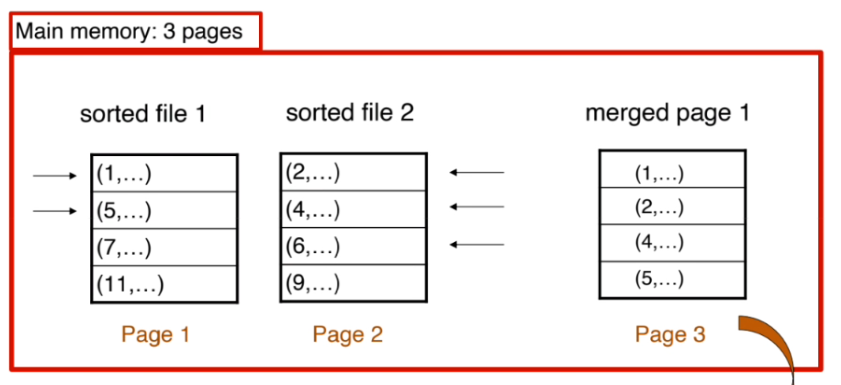
\includegraphics[width=0.7\linewidth]{img/screenshotss001}
		\caption{外部排序}
		\label{fig:screenshotss001}
	\end{figure}
	\item \textit{Question}:如果文件(pages)未排序,该如何排序?
	\begin{itemize}
		\item 情况一:文件页数小,放入主存用任意排序算法排序。
		\item 情况二:文件页数大,无法放入主存进行排序:
		\begin{enumerate}
			\item 将数据逐批带入主存,每一批都是$M$页,使用主存排序算法排序后写回。
			\item 迭代的对上述排序文件进行$M-1$路合并。(需要1页写出排序结果)
		\end{enumerate}
		\item 未排序大文件例子:$M=4page$,1个大文件,每个文件有100个page
		\begin{figure}[th]
			\centering
			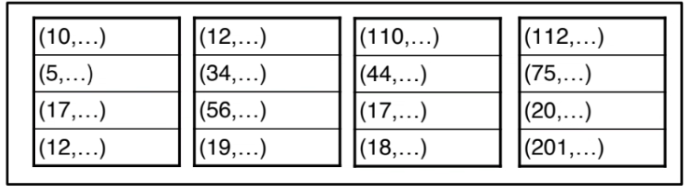
\includegraphics[width=0.5\linewidth]{img/screenshotss002}
			\caption{未排序大文件}
			\label{fig:screenshotss002}
		\end{figure}
		\begin{enumerate}
			\item 
			分$100/M=25$批,每次读取$M=4$页进行排序,得到$a_1$至$a_{25}$个文件。
			\item 对上述25个文件进行$M-1=3$路合并,每次合并三个,迭代直到结束。 
		\end{enumerate}
		\begin{figure}[th]
			\centering
			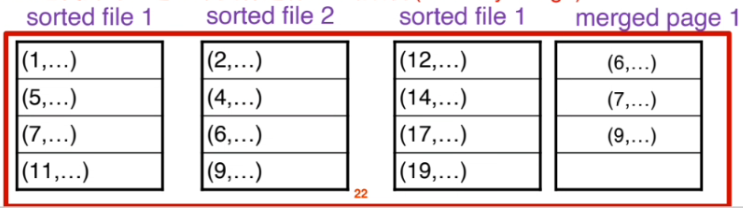
\includegraphics[width=0.5\linewidth]{img/screenshotss003}
			\caption{合并排序好的子文件}
			\label{fig:screenshotss003}
		\end{figure}
	\end{itemize}
	\item 外部排序算法总结:
	\begin{itemize}
		\item[$\rightarrow$] $M$:主存大小(page);$R$:关系表;$b_r$:存储整个$R$
		需
		要
		的页数
		\item 阶段一:读取关系表中的$M$页进入主存并排序,从而得到$N$个子表$R_i$。
		\item 阶段二:如果$N\leq M-1$,则直接N-way合并。如果$N\geq 
		M$,则连续合并$M-1$个文件,一个pass将文件个数减少$M-1$倍,同时长度增大$M-1$倍
		,直到所有文件合并为一个文件。成本为$b_r(2\lceil \log_{M-1}(b_r/M)\rceil 
		+1)$。
	\end{itemize}
	\begin{figure}[th]
		\centering
		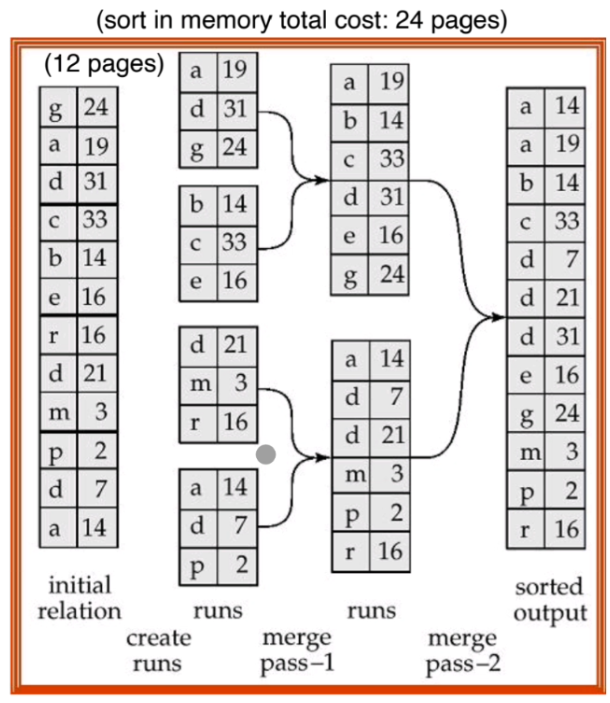
\includegraphics[width=0.7\linewidth]{img/screenshotss004}
		\caption{整体外部排序例子}
		\label{fig:screenshotss004}
	\end{figure}
	
\end{itemize}

\section{连接算法}

\textbf{连接算法引入}
\begin{itemize}
	\item 连接算法即Join algorithms。
	\item 连接算法的成本只简单考虑I/O次数,即page读写次数。
	\item \textit{Notation}:
	\begin{itemize}
		\item $r,s$:两个连接的关系表。
		\item $n_r,n_s$:$r$和$ s $的记录数。
		\item $ b_r,b_s $:$r$和$ s $的页数。
		\item $ \mathbf{M} $:内存的可用页数。
	\end{itemize}
\end{itemize}

\begin{figure}[th]
	\centering
	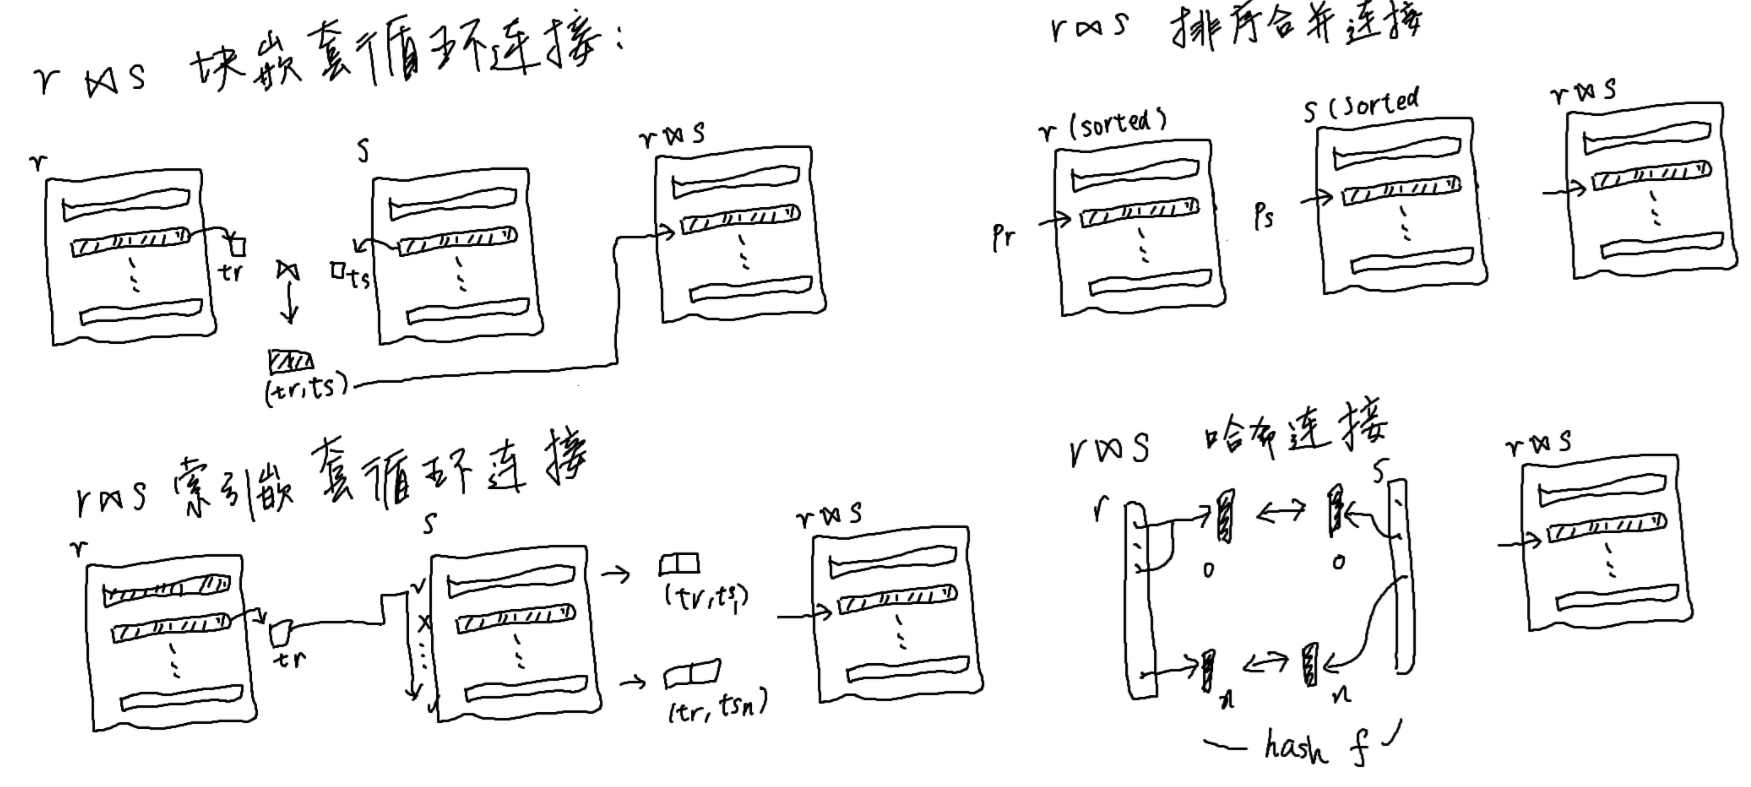
\includegraphics[width=0.9\linewidth]{img/1321screenshot001}
	\caption{四种连接算法图示}
	\label{fig:1321screenshot001}
\end{figure}

\textbf{连接算法复杂度分析}
\begin{itemize}
	\item 块嵌套循环连接:
	\begin{itemize}
		\item 最坏成本:$b_r*b_s+b_r$。(主存的页面大小=3页)\\对于$ r $的每一个页面都遍历一
		次$ 
		s 
		$。也就是要把$ r $里面的每一个页面依次主存,每一次把$ s $的所有页面再依次
		读入主
		存,即$ b_r*b_s $。最后一项$ b_r $是写输出成本。
		\item 最好成本:$ b_r+b_s $ 可以把整个$ r $都都进去主存。
		\begin{figure}[th]
			\centering
			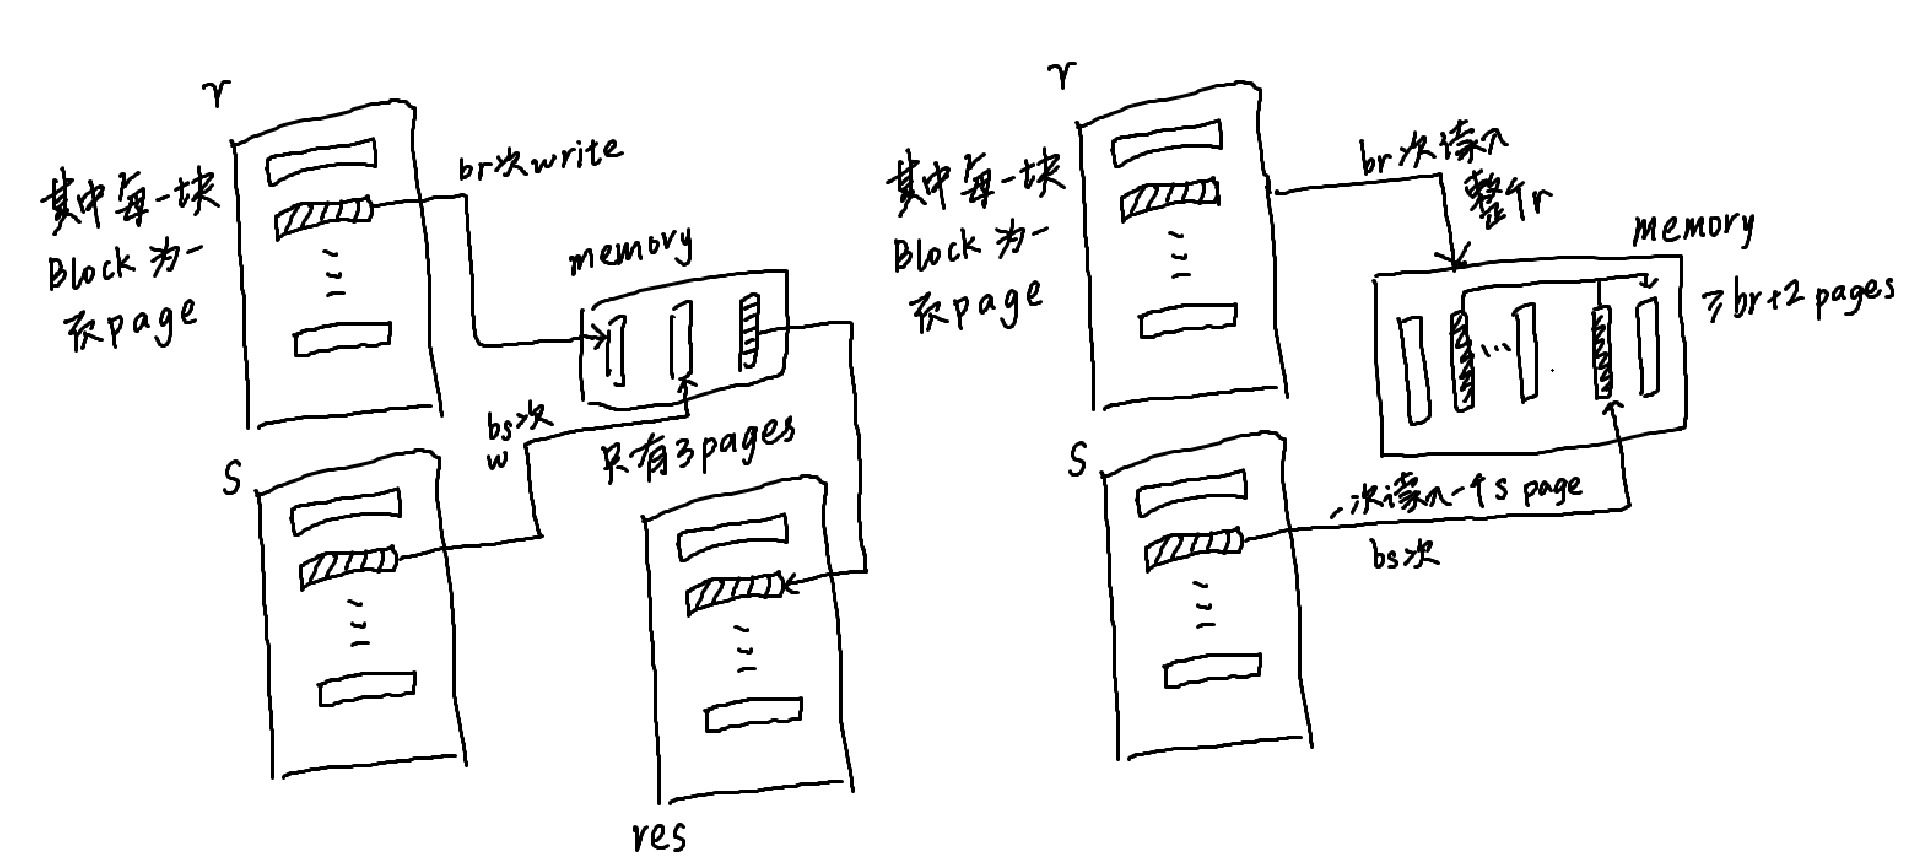
\includegraphics[width=0.7\linewidth]{img/db1}
			\caption{块嵌套循环连接时间复杂度分析}
			\label{fig:db1}
		\end{figure}
		
		\item 一般情况:使用$ M-2 $内存页面存储外关系$ r $的pages,剩下的2页一页用于
		读取$ s $,一页用于写输出。总成本为$ \lceil b_r/(M-2)*b_s \rceil+b_r$。
		\begin{figure}[th]
			\centering
			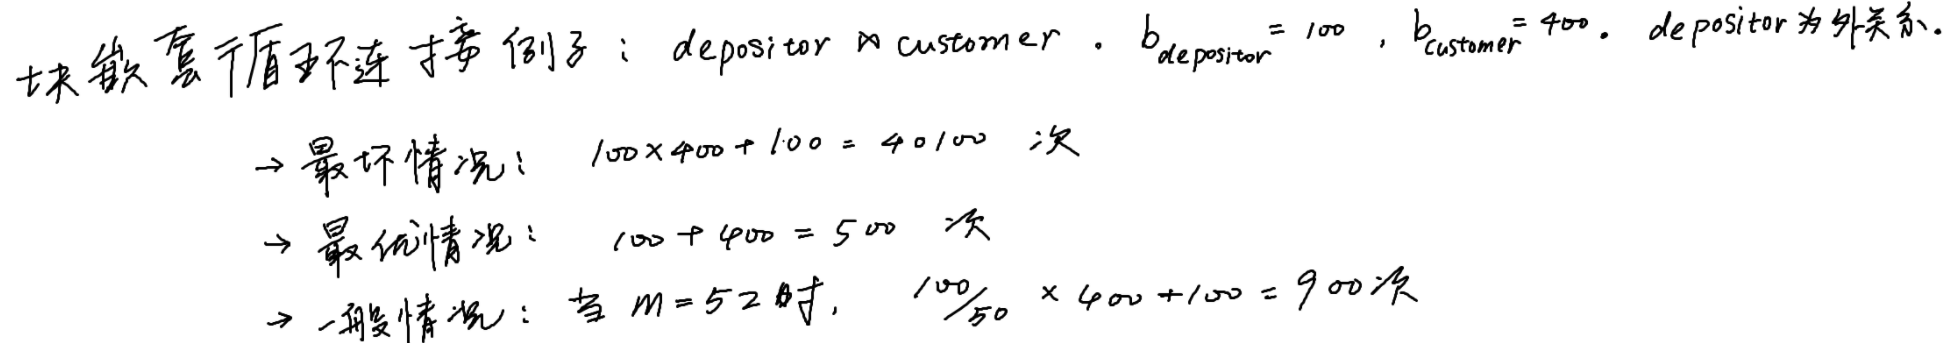
\includegraphics[width=0.7\linewidth]{img/dsdsascreenshot001}
			\caption{块嵌套循环连接例子}
			\label{fig:dsdsascreenshot001}
		\end{figure}
		
	\end{itemize}
	\item 索引嵌套循环连接:
	\begin{itemize}
		\item (...)
	\end{itemize}
\end{itemize}

\section{查询优化}

\textbf{Intro}:查询优化不只是计算每个运算的成本,并且需要考虑不同操作执行步骤间在输入
输出的交互。

\textbf{系统目录信息}:存储描述数据的数据
\begin{itemize}
	\item 对于关系表$ R $:$ n_R $标识元组数量,$ b_R $标识页面数量。
	\item 额外信息:
	\begin{itemize}
		\item $ f_R $一个页面能容纳的元组数量,$ b_R=\lceil 
		n_R/f_R\rceil $。
		\item $ V(A,R) $:$ R $中属性$ A $的不同值数量,即$ \pi_A(R) $的大小。
	\end{itemize}
	\item 对于每个索引$ i $,系统存储以下信息:
	\begin{itemize}
		\item $ HT_i $:索引$ i $的层数,即索引树的高度。
		\begin{itemize}
			\item 对于关系表$ R $,根据属性$ A $构建的树,高度$ HT_i = \lceil 
			\log_{f_i}(V(A,R)) \rceil $。
			\item 对于哈希索引,如果我们设定了溢出桶,则$ HT_i = 1.x $;否则$ HT_i 
			= 1 $。
		\end{itemize}
			\item 额外信息:
		\begin{itemize}
			\item $ f_i $:内节点的扇出数(fanout)。
			\item $ LB $:叶节点占用的页面数量。
		\end{itemize}
	\end{itemize}
\end{itemize}

\begin{smallmdframed}
	以上包括关系表的信息、页面的信息、属性的信息以及索引的信息。\\
	用以上信息来刻画选择大
	小估计表达式
	。
\end{smallmdframed}

\textbf{选择大小估计 Selection Size Estimation}  
\\一次操作的输出大小决定了该操作的成本以及后续操作的成本。其准确估计对于优化很重要。
\begin{itemize}
	\item {Equality selection} $\sigma_{A=v}(R)$  
	例如:$\sigma_{\text{rating}=8}(\text{SAILORS})$
	\begin{itemize}
		\item 定义$ SC(A,R) $:属性$ A $在关
			系表$ R 
		$上的选取数目。
		\item $ A $上满足一个等式的记录的平均数:$ SC(A,R) = 
		\frac{n_R}{V(A,R)} $
		\item $\lceil SC(A,R)/f_R \rceil$:如果这些记录按属性$ A $排序,存储这
		些记
		录所需的页/块数。
		\item 如果记录在$ A $上没有排序,则每条记录可能驻留在不同的页面中。
		\item 特殊情况:如果$ A $是{关键属性},则$ SC(A,R) = 1 $。
	\end{itemize}
\end{itemize}

\textbf{Selections Involving Comparisons}  
\\选择形式:$\sigma_{A<v}(R)$(同理可分析$\sigma_{A>v}(R)$的情况)  
令$ S $表示满足条件的元组的估计数量:$ \min(A,R) $和$ \max(A,R) $可以从
目录中获得。

假设属性A的值是均匀分布的:
\[
S =
\begin{cases}
	0, & \text{if } v < \text{min}(A,R) \text{ 或 } v > \text{max}(A,R) \\
	n_R \cdot \frac{v - \text{min}(A,R)}{\text{max}(A,R) - \text{min}(A,R) 
	+ 1}, & \text{otherwise}
\end{cases}
\]

{Example:}  
$$
\sigma_{\text{rating}<2}(\text{SAILORS}) = \text{\# records in sailors} \cdot 
\frac{2-1}{10-1+1}= \text{\# records in sailors} / 10
$$
\\使用{直方图}能得到更准确的估计。本质上是概率统计的一个过程,暂不展开。

\textbf{等价关系表达式}:有很多表达式的结果是等价的,我们称其为等价表达式。
\begin{itemize}
	\item 选择操作的交际可以结构为单独选择,且选择是可交换的。
	\item 在序列投影操作中只需要保留最后一个,其他的投影操作可以省略。
	\item 选择条件可以嵌入到叉积或连接里面。
	\item 连接操作是可交换、元素可结合、选择条件可结合的。
	\item 在以下两个条件中,选择操作可以前置于theta join操作上。
	\begin{itemize}
		\item 当$ \theta _1 $只涉及$ E_1 $表中的属性,$ \theta _2 $只涉及$ E_2 $表
		中的属性:\\
		$\sigma_{\theta1\wedge\theta2}(\mathbb{E}_1\Join_\theta\mathbb{E}_2)=(\sigma_{\theta1}(\mathbb{E}_1))\Join_\theta(\sigma_{\theta2}(\mathbb{E}_2))$
	\end{itemize}
	\begin{smallmdframed}
		在数据库中,Theta Join(θ连接) 是一种基于条件的连接操作,用于将两个表按照特定
		的条件组合在一起。与等值连接(Equi-Join)不同,Theta Join 可以使用任意比较运
		算符,而不仅仅是等于运算符 (=)。
	\end{smallmdframed}
\end{itemize}
目前查询优化器包含一下两种主要方法:
\begin{itemize}
	\item 启发式算法优化:尽早执行选择,尝试利用检索,删除无用属性
	\item 基于成本的优化:估算所有计划,选择最优计划。
\end{itemize}

\textbf{启发式算法优化}
\begin{itemize}
	\item 尽早执行选择操作:当$ \theta _1 $只涉及$ E_1 $表中的属性,$ \theta _2 $只
	涉及$ E_2 $表
	中的属性:\\
	$\sigma_{\theta1\wedge\theta2}(\mathbb{E}_1\Join_\theta\mathbb{E}_2)=(\sigma_{\theta1}(\mathbb{E}_1))\Join_\theta(\sigma_{\theta2}(\mathbb{E}_2))$
	
	\item 尽早执行投影操作:$ \pi_a(R \Join S) = \pi_a((\pi_{a1} R) \Join 
	(\pi_{a2} S)) $
\end{itemize}

\textbf{基于成本的优化}
\begin{itemize}
	\item $ n $个连接操作($ n+1 $个关系表)可能得到的连接树数量为:$ (2n)!/n! $。
	\begin{itemize}
		\item 连接树的形状数量为:$ (2n)!/[n!(n+1)!] $。
		\item 每棵树共有$ (n+1)! $种排列方式。
	\end{itemize}
	\item 子序列会重复评估,将所有可能子序列写进内存后直接提取。
	\begin{enumerate}
		\item[$\Rightarrow$] 思路:所有执行计划都可以用$ S_1\Join(\mathbf{S}-S_1) 
		$来表示,递归求解。
		\item 枚举$ \mathbf{S} $中的所有非空子集$ S_1 $
		\item cost=cost($ S_1 $)+cost($ \mathbf{S}-S_1 $)+cost($ 
		S_1\Join(\mathbf{S}-S_1) $)
		\item 选择cost最少的plan
	\end{enumerate}
	\item 成本仅计算将中间结果协会磁盘的cost
	\item \textit{这一部分没看懂。以后搞懂。}
\end{itemize}

\section{Transactions事务处理}
事务是访问并可能更新各种数据项的程序执行单元。

\textbf{事务的性质}:ACID,原子、一致(顺序无关)、隔离(过程不可见)、持久(保持)

\newpage
\tableofcontents
\label{toc}
\appendix
\newpage

\section{作业二}
苏睿熹 22330100\\
\textbf{Part 1. Convert the ERD into the corresponding database schema:}

(Underline the primary keys and foreign keys.)

对于同一种情况(如关系的映射),课件中可能讨论了多种做法,如果课件中没有明确说哪种会最优
的,皆以ppt出现的第一种做法为准。

\begin{figure}[ht]
	\centering
	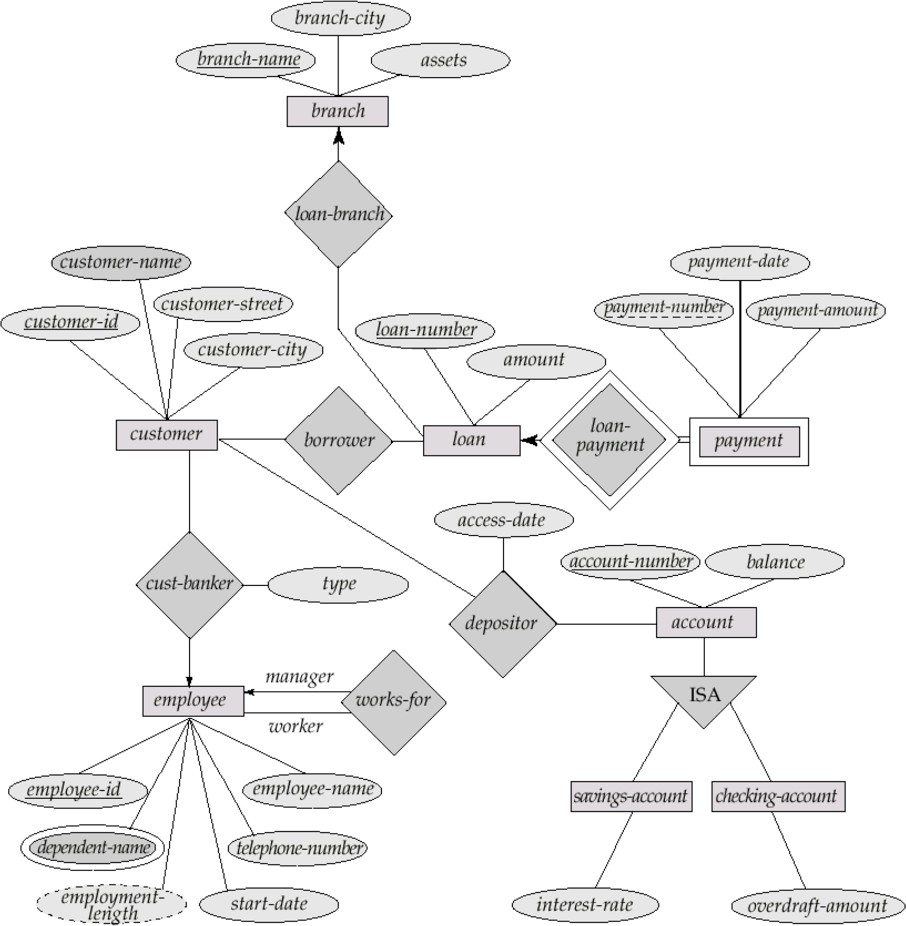
\includegraphics[width=0.7\linewidth]{img/图片1.png}
	\caption{Part 1 ERD}
	\label{fig:my_label}
\end{figure}

\begin{enumerate}
	\item 为强实体集构建相应的relations:
	\begin{itemize}
		\item[$\Rightarrow$] BRANCH:\underline{branch-name} $\|$ branch-city 
		$\|$ assets
		\item CUSTOMER:\underline{customer-id} $\|$ customer-name $\|$ 
		customer-street $\|$ customer-city
		\item EMPLOYEE:\underline{employee-id} $\|$ start-date $\|$ 
		telephone-number $\|$ employee-name
		\begin{smallmdframed}
			由于employment-length为衍生属性,所以不创建相应属性以避免数据不一致。\\由
			于dependent-name为多值属性,所以多创建一张表DnTable。
		\end{smallmdframed}
		\item[$\Rightarrow$] DNTABLE:\underline{employee-id} $\|$ 
		dependent-name
		\item LOAN:\underline{loan-number} $\|$ amount
		\item[$\Rightarrow$] ACCOUNT:\underline{account-number} $\|$ balance
	\end{itemize}
	\item 为弱实体集创建相应的relations:
	\begin{itemize}
		\item PAYMENT:\underline{loan-number} $\|$ \underline{payment-number} 
		$\|$ payment-date $\|$ payment-amount
	\end{itemize}
	\item 构建1-to-1关系:图中没有。
	\item 构建1-to-many关系:
	\begin{itemize}
		\item[$\Rightarrow$] LOAN:\underline{loan-number} $\|$ amount $\|$ 
		branch-name
		\item[$\Rightarrow$] PAYMENT:\\\underline{loan-number} $\|$ 
		\underline{payment-number} 
		$\|$ payment-date $\|$ payment-amount $\|$ loan-number
		\item[$\Rightarrow$] CUSTOMER:\\\underline{customer-id} $\|$ 
		customer-name $\|$ 
		customer-street $\|$ customer-city $\|$ employee-id $\|$ type
		\item[$\Rightarrow$] EMPLOYEE:\\\underline{employee-id} $\|$ 
		start-date $\|$ 
		telephone-number $\|$ employee-name $\|$ manager-id
	\end{itemize}
	\item 构建many-to-many关系:
	\begin{itemize}
		\item[$\Rightarrow$] BORROWER:\underline{customer-id} $\|$ 
		\underline{loan-number}
		\item[$\Rightarrow$] DEPOSITOR:\underline{account-number} $\|$ 
		\underline{customer-id} $\|$ access-date 
	\end{itemize}
	\item 构建层级模型:
	\begin{itemize}
		\item[$\Rightarrow$] SAVINGACC:\underline{account-number} $\|$ 
		interest-rate
		\item[$\Rightarrow$] CHECKINGACC:\underline{account-number} $\|$ 
		overdraft-amount
	\end{itemize}
\end{enumerate}

在上述过程中,\underline{由箭头$\Rightarrow$指向的关系表为最终构建结果}。

\textbf{Part 2. 3NF and BCNF Decomposition:}
\\Schema $R=(A,B,C,D,E)$ with $F=\{AB\rightarrow C, A\rightarrow D\}$
\\1. DO the \underline{3NF Decomposition}
\begin{itemize}
	\item 所有的候选键位:$A$,$B$和$E$。
	\item 不满足2NF,因为存在部分依赖$A\rightarrow D$。进行2NF分解:
	\begin{itemize}
		\item $R\Rightarrow R_1=(A,B,C), R_2=(A, D), R_3=(A,B,E)$
		\item 不存在传递依赖,满足3NF。
	\end{itemize}
\end{itemize}
2. DO the \underline{BCNF Decomposition}
\begin{itemize}
	\item $R\Rightarrow R_1=(A,B,C), R_2=(A, D), R_3=(A,B,E)$
	\item $R$ 是在 BCNF 中当且仅当对于每个函数依赖 $X \rightarrow \{A\}$ 在 $F^+$ 
	中,至少满足以下两个条件的其中一条:
	\begin{itemize}
		\item $A \in X$(函数依赖是平凡的)。
		\item $X$ 是R的超键。
	\end{itemize}
	\item 分解后满足BCNF。
	\item 不会丢失函数依赖。
\end{itemize}
\label{toc}

\newpage
\section{Tutorial 7: Indexing\&$ B^+ $tree\&Hashing}

\textbf{内容回顾:}索引的目的是为了加速对需要数据的获取速度。其中比较重要的概念是\underline{
搜索键},即用于记录搜索的属性。索引分为顺序索引和哈希索引两种。

索引的特征可分为三项:主要/辅助,密集/稀疏,单层/多层。Primary指的是搜索键顺序刚好和文
件排列顺序一致,密集指的是一条index只对应一个记录,多层索引即可以为索引创建索引。

\textbf{Exercise 1:}
\begin{figure}[th]
	\centering
	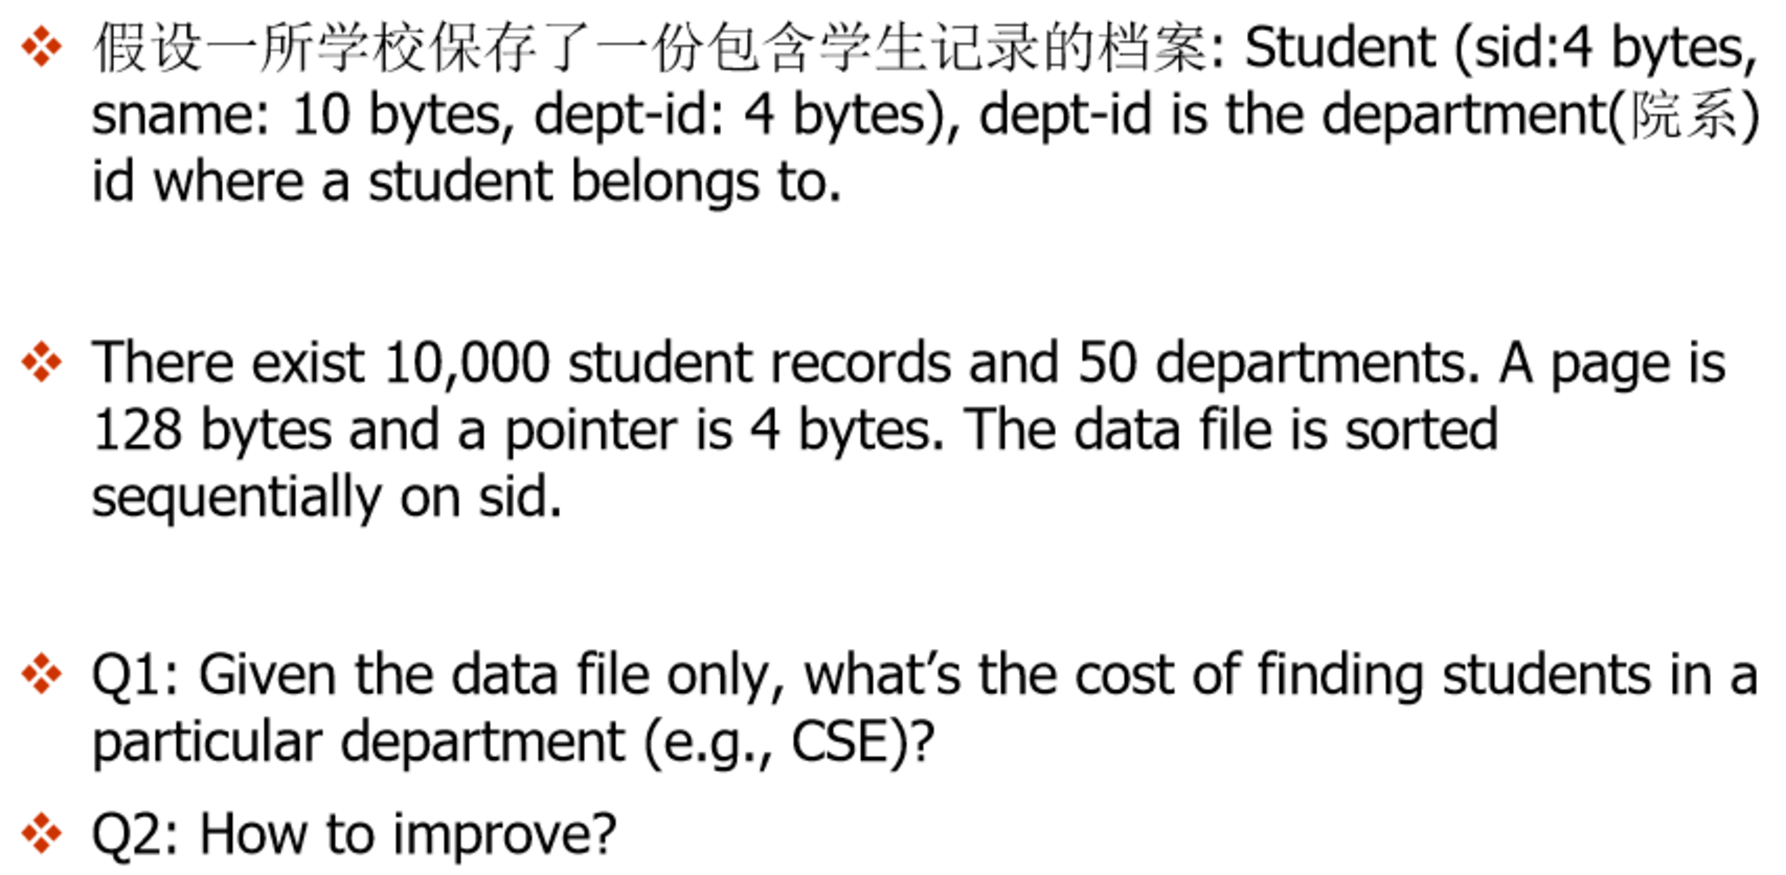
\includegraphics[width=0.7\linewidth]{img/dsdsascreenshot002}
	\label{fig:dsdsascreenshot002}
\end{figure}

\textbf{Q1:}由于数据文件是用sid进行排序的,所以要检索特定department的记录,需要自上
而下的检索一遍所有页面。一条学生记录占用18bytes,
一共有10000
个学生记录。一个页面最多可以存储记录数量为:$\lfloor128/18\rfloor =7$,又因为
$\lceil 10000/7 \rceil = 1429$,所以一共要读取1429次磁盘页面。
\begin{smallmdframed}
	如果记录可以跨页存储,则只需要$\lceil 10000*18/128 \rceil = 1407$次。
\end{smallmdframed}

\textbf{Q2:}构造一个关系实体,存储department和pointer之间的对应关系(department, 
pointer)。每一条记录为8bytes。顺序索引和哈希索引的不同开销分析如下:
\\假设每个department刚好有200个students。
\begin{itemize}
	\item 顺序索引:	
	\item 哈希索引:
\end{itemize}

\textbf{Exercise 2:$ B^+ $ tree:}
\begin{figure}[th]
	\centering
	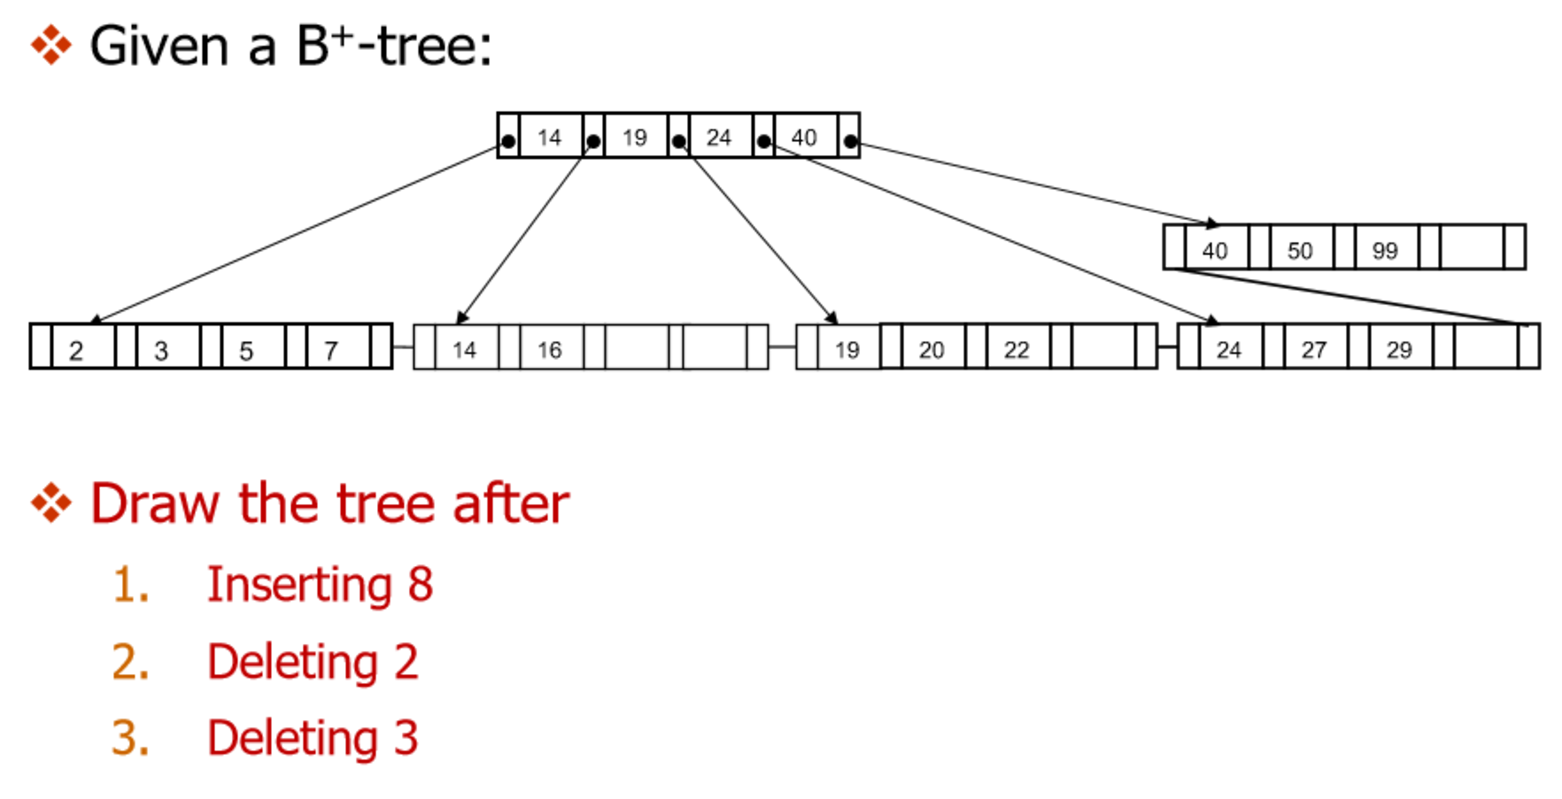
\includegraphics[width=0.7\linewidth]{img/dsdsascreenshot003}
	\label{fig:dsdsascreenshot003}
\end{figure}

\textbf{插入8:}
\begin{figure}[th]
	\centering
	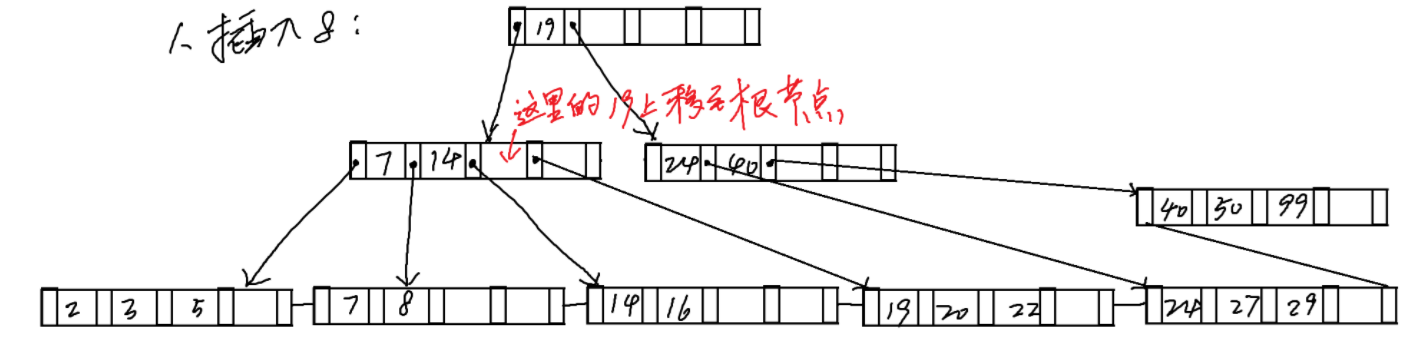
\includegraphics[width=0.7\linewidth]{img/dsdsascreenshot004}
	\label{fig:dsdsascreenshot004}
\end{figure}


\end{document}
